\graphicspath{{chapter_1}}
\chapter[Marker-free Unified Eye-Hand Calibration]{Marker-free Unified Eye-Hand Calibration}
\chaptermark{Marker-free Unified Eye-Hand Calibration}
\label{chap:registration}
\minitoc

\paragraph{Disclaimer} This \chapref{chap:registration} is an \textit{in extenso} reproduction of work
%submitted
prepared
for consideration in a journal publication.
%to IEEE Transactions on Biomedical Engineering, which is currently under review.
Only \secref{c1:sec:introduction} is altered to highlight additional context within the scope of this thesis and remove redundancy with \chapref{chap:introduction}.
%\secref{in:sec:spatial_awareness}, \secref{c1:sec:robust_icp}, and \secref{in:sec:marker_free_unified_calibration} were discussed in \chapref{chap:introduction} to form a consistent picture.

\newpage

\section{Introduction}
\label{c1:sec:introduction}
Multi-robot arm systems possess an incredible potential to revolutionize the way we approach complex tasks, improving efficiency and productivity. 
By utilizing multiple arms, we can overcome the limitations of a single unit, extending the range of possible tasks that the system can perform. 
For example, suturing requires at least two arms.
There exists a wide variety of multi-robot arm applications beyond surgical robotics including 
agriculture~\cite{Xiong20}, 
civil engineering~\cite{Yasutomi23}, 
space robotics~\cite{Yan20},
packaging and assembly~\cite{Do12},
nuclear decommissioning~\cite{Mohamed07},
disaster recovery~\cite{Kamezaki16}, and
sub-sea robotics~\cite{Brantner21}.

%The da Vinci\textsuperscript{\textregistered} system by Intuitive Surgical Inc. is widely regarded as an example of a successful surgical robot system~\cite{yang2018grand, DEttorre2021} utilizing four robot arms (three for manipulation and one for imaging). However, due to its large size, incorporating the da Vinci system into the operating theater becomes arduous, restricting patient access, and making it cumbersome to remove in the event of manual intervention being required.Recently, alternative platforms have emerged that adopt a modular design where the robot arms are mounted on mobile platforms or the surgical table. 
%Examples include the 
%DLR MIRO research platform~\citep{miro}
%as well as commercial systems such as 
%the Senhance\textsuperscript{\texttrademark} Surgical System by Asensus Surgical, 
%the Hugo\textsuperscript{\texttrademark} \gls{ras} System by Medtronic, 
%the Versius\textsuperscript{\textregistered} Surgical System by \gls{cmr} Surgical, and 
%the SSI Mantra by SS Innovations.

Direct teleoperation, classified as level zero in the taxonomy proposed by Yang et al.~\cite{Yang2017}, is a control approach that maps signals from a surgeon-device interface onto robot motion~\cite{Niemeyer2008}, typically using position/velocity based commands.
Currently, direct teleoperation is the gold-standard for the majority of surgical robotic systems in use today. This approach guarantees that the operating surgeon is solely responsible for the robot's motion, emphasizing the need for skilled training and practice~\cite{Liu15}. Lack of training, as explained in the introductory \secref{in:sec:spatial_awareness}, may lead to severe surgical workflow interruptions. Collision models and collision avoidant control is thus desirable. A prerequisite to collision avoidant control, however, is precise localization. With the increasing automation of surgical procedures, e.g. see recent work by Saeidi et al~\cite{Saeidi2022}, the demand for localization strategies and collision models becomes even more pronounced.

% As a result, the system integration forgoes the requirement for a collision model in these multi-arm setups. 

A key requirement for future automated systems is robot base-to-base localization, i.e. each robot arm must be aware of the other arm's position and orientation with respect to its own. This is needed in order to implement an effective collision model into the automated control system ensuring patient and the operating team's safety. In the case where multi-robot arm systems are deployed on a surgical table, base localization can be derived from \gls{cad} models, however, these measurements may not accurately reflect reality due to manufacturing inaccuracies. In the case of the increasingly popular modular systems, mentioned in \secref{in:sec:robot_surgery_platforms}, the arm setup may be different every time the theater is prepared. Furthermore, robotic systems must also undergo localization in relation to other elements present in the operating theater, including patient anatomy, lighting fixtures, imaging systems (e.g. C-arm), and so on, see \figref{in:fig:room_setup}. This motivates the need for a robot base calibration step introduced into the surgical workflow. Such a step, however, should be designed in a way that can be quickly and safely performed by non-robotics experts, i.e. the theater staff.

% The development of commercialized RGBD camera devices has been  

% Knowledge of the robot base-to-base localization is especially important in the case of the modern modular systems mentioned above.
% However, it can also be important for systems mounted on the surgical table since the measurements from \gls{cad} models may not reflect reality due to .
% need to recalibrate for modern modular systems 
% especially in the case of the modern modular systems mentioned above
% furthermore, the calibration process needs to be simplified so that it can be performed quickly by non-robotics experts
% even in case of robots being deployed on a surgical table, the \gls{cad} models may need not fully reflect reality

% Surgical robotics has become a key tool for improving patient outcomes.

% Reduced physical stress on surgeons~\citep{}.
% Reduced forces applied to trocars~\citep{} reducing damage to the incision points thus reducing recovery time, need a reference.
% Finer control/dexterity for certain tasks, e.g. suturing~\citep{}, spine 
% Furthermore, surgical robotics can enable autonomous surgery~\citep{}

% The established paradigm for surgical robots is to have a monolithic device which integrates all robot arms into a single connected device. Example systems that have adopted this design are the da Vinci\textsuperscript{\textregistered} by Intuitive Surgical, the avatera\textsuperscript{\textregistered} by avateramedical, and the hinotori\textsuperscript{\texttrademark} by Medicaroid. These are inflexible for use in the operating room, restrict patient access and are difficult to remove should the need arise for manual intervention.

% To improve flexibility, other surgical robotics platforms have adopted a new modular design paradigm where the robot arms are mounted on individual mobile platforms or the surgical table. Examples are the  DLR MIRO~\citep{miro} research platform as well as commercial systems such as the Senhance\textsuperscript{\texttrademark} Surgical System by Asensus Surgical, the Hugo\textsuperscript{\texttrademark} \gls{ras} System by Medtronic, the Versius\textsuperscript{\textregistered} Surgical System by \gls{cmr} Surgical, and the SSI Mantra by SS Innovations.

%While providing numerous benefits, the distributed paradigm brings its own issues, primarily the unknown location of the robots with respect to each other and with respect to the surgical setup. 

%- spine to robot registration
%- camera to robot registration
%- greatly simplifying setup
%- building a world map (providing a better world model)
%- robot to whatever registration for collision free path

%WHAT TASKS IN HUMAN CONTROLLED ROBOTIC SURGERY REQUIRE GOOD BASE-TO-BASE REGISTRATION?

%Autonomous surgery needs accurate base-to-base.

%This paper focuses on solving this problem



%\begin{figure}[tbh]
%\centering
%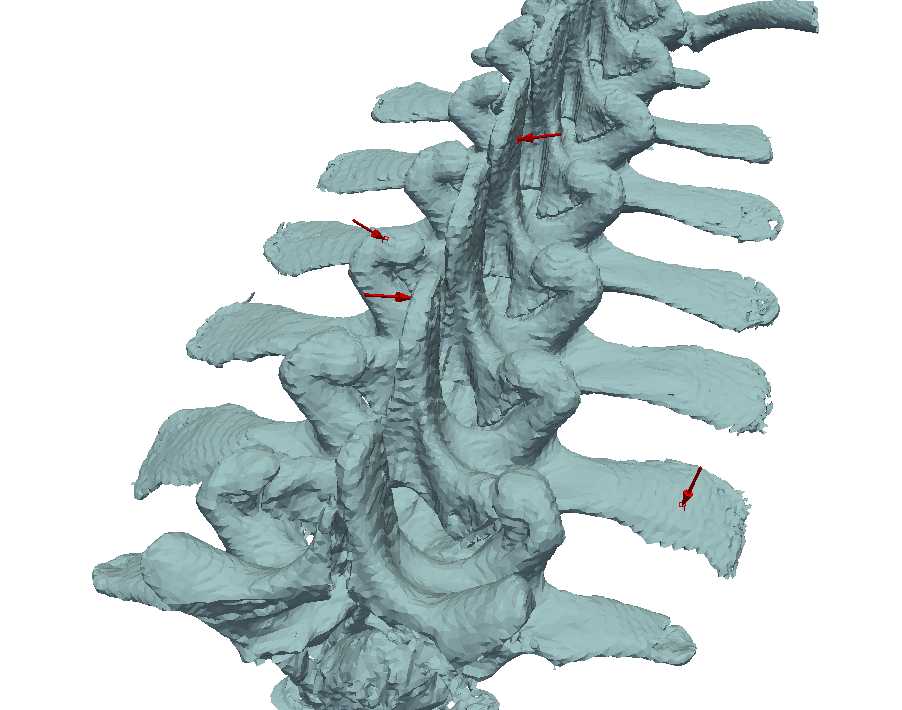
\includegraphics[width=0.45\columnwidth]{fig/preop_plan}
%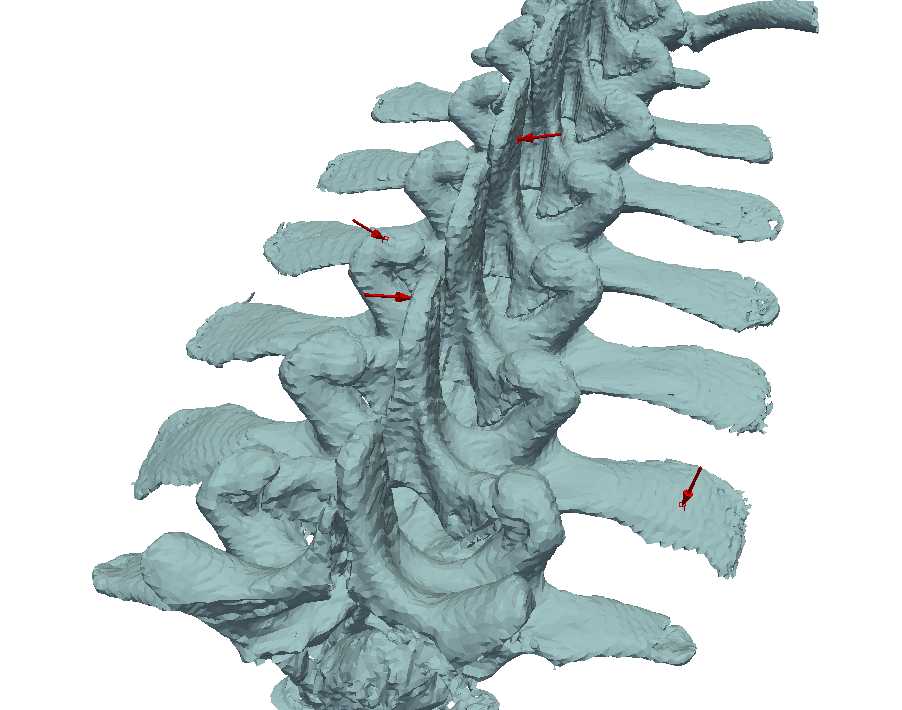
\includegraphics[width=0.45\columnwidth]{fig/preop_plan}
%\caption{The preoperative plan (left) and the corresponding surgical site (right). The arrows on the left-hand image show the planned imaging targets that will be executed by the robot.} 
%\label{c1:fig:preop_plan}
%\end{figure}



\subsection{Contributions}
\begin{figure}[tb]
    \centering
    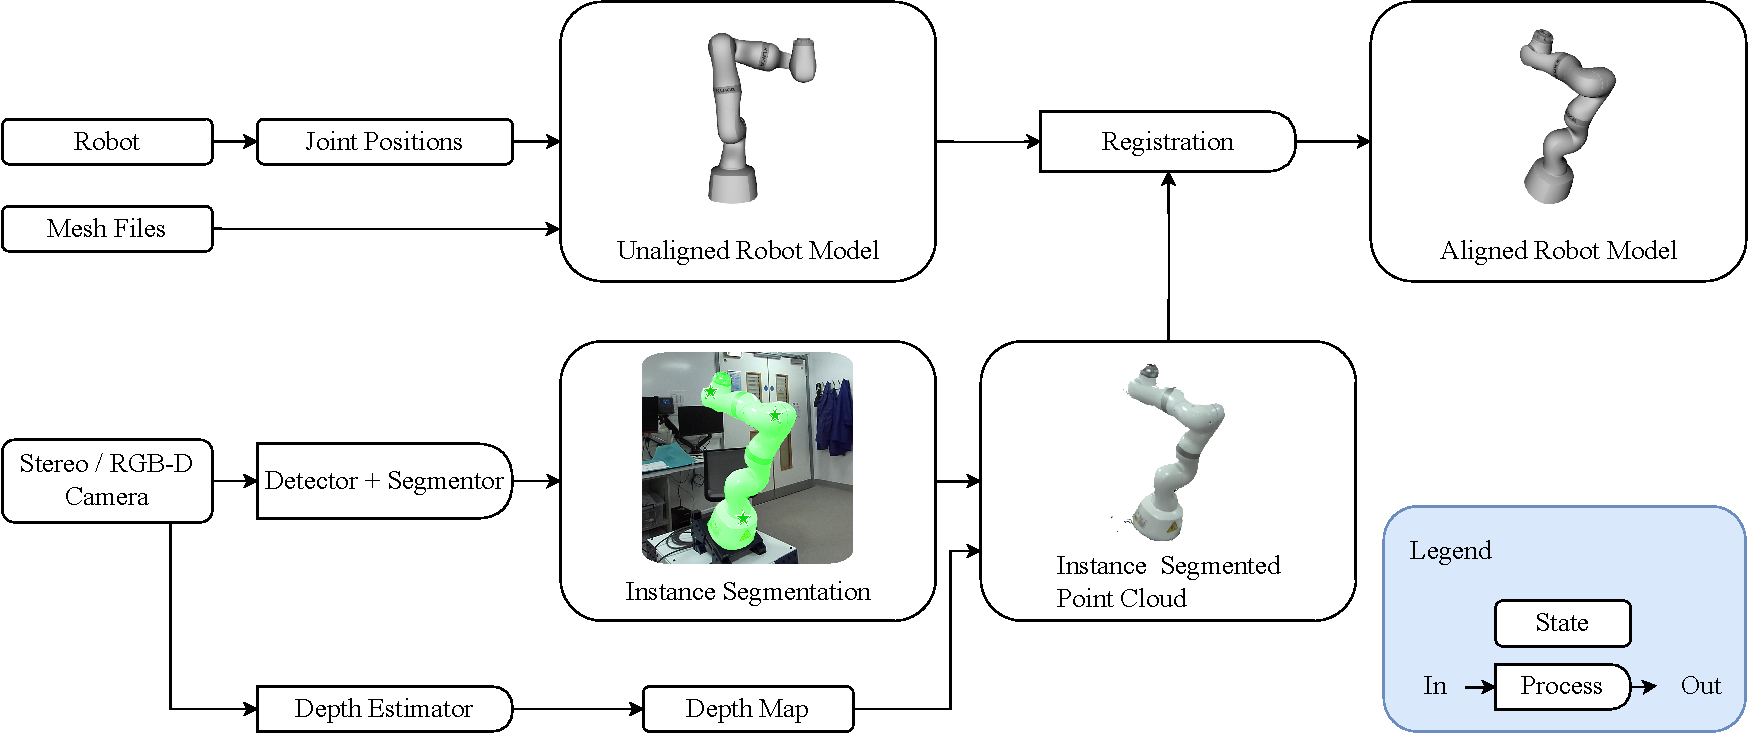
\includegraphics[width=\textwidth]{chapter_1/fig/approach_refined.pdf}
    \caption{Proposed registration procedure. The pipeline takes joint positions and corresponding stereo or RGB-D images as input and yields eye-to-hand transformations. Upper half: Joint positions from the robot(s) are used to transform the link mesh files into an unaligned robot model. Lower half: Stereo (or RGB-D) images are fed through a depth estimator to obtain a depth map. A monocular image is taken from the stereo image and is used to detect and instance segment the robot. The depth map and instance segmentation are fused to obtain an instance-segmented point cloud. The instance-segmented point cloud is registered to the unaligned robot model to obtain a robot model that is aligned with the observed image. The transform from unaligned to aligned robot model describes the robot to camera homogeneous transform $\homogeneous{C}{B}$. Refers to \secref{c1:sec:proposed_calibration_procedure}.}
    \label{c1:fig:calibration_pipeline}
\end{figure}
In this work we make the following contributions:
\begin{itemize}
    \item A unified approach for eye-in-hand and eye-to-hand calibration of multiple surgical robots with no need for any calibration targets since the robot itself is used instead. Our proposed method uses a novel robust \gls{icp} formulation of a point-to-plane objective on a Lie algebra. Only RGB-D images, the robots' joint positions, and their respective mesh files or \gls{cad} models are used.
    \item We conduct several benchmarks comparing our methods against classical approaches. Our method ensures safety and, based on the comparisons, demonstrates faster execution and better outcomes when compared to other options.
    \item Hardware realization of the approach on a dual robot arm system. Furthermore, we showcase a human-robot collaboration through admittance control with arm-arm collision avoidance. The collision model for the two robots relies on the measurements generated by our proposed method.
    %The two robots are controlled in a collision avoidant manner.
    % Upon acceptance of this manuscript, our intention is to make the code-base publicly available as an open-source contribution. This will encompass both the proposed method itself and the \gls{phri} controller, that includes integrated collision avoidance functionality.
    \item We conduct an in-vivo experiment in a clinically relevant dual-arm setup for spine surgery.
\end{itemize}

% We present a method of providing base-to-base registration for two or more surgical robots using a stereo or RGB-D camera. The method uses the current joint states of each arm to configure the arm's mesh, which is then fitted to the point cloud using the Iterative Closest Point (ICP) method.
% We compare our results to handshaking and show our results to be comparable while taking much less time to perform.


% It provides a unified approach to eye-in-hand and eye-to-hand calibration and does not require any calibration targets, since it uses the robot as calibration target itself.

\section{Related Work}
\subsection{Eye-in-hand Calibration}
Prior work on the eye-in-hand problem~\cite{Horaud95, Strobl06} require the user to fabricate a marker (e.g. checkerboard or AprilTag~\cite{Olson11}) with known geometry making it easy to extract a pose from images. In our work, we do not require the user to create such a marker.
Instead, we make use of the mesh files or \gls{cad} models provided by the manufacturer.

\subsection{Marker-free Registration}
Marker-free eye-to-hand calibration is an active research field with new developments being lead by differentiable rendering frameworks, such as PyTorch3D~\cite{ravi2020pytorch3d} and Kaolin~\cite{KaolinLibrary}. Consequentially, some works utilize these frameworks to optimize for camera poses such that mesh renders match image segmentations~\cite{Chen:RAL:2023}. Further work proposes a fully self-supervised procedure that learns both, to segment and to estimate the eye-to-hand transformation~\cite{lu2023markerless}. These works require tailoring to dedicated robot models and depend on fully-blown differentiable rendering pipelines, which makes them difficult to use in practise. Other work that doesn't use differentiable rendering but rendering is~\cite{labbe2021single}, where the authors also predict joint states on top of the eye-to-hand registration. This work also requires training to dedicated systems. Simpler approaches suggest to predict robot joint positions and extract eye-to-hand registrations through solving a \gls{pnp} problem~\cite{lee2020camera}. In this work, we suggest a conceptually much simpler approach that works for any robot, but uses RGB-D images, and, as some of the other methods, robot joint states. Closest to our work comes~\cite{point_cloud_based_robot_cell_calib}, where the authors also perform point cloud registration. Their method, however, only registers a single configuration and performs complex clustering of the observed point cloud. The only marker-free work on a surgical system is presented in~\cite{hand_eye_calibration_robotic_assisted}, where the authors utilize the surgical tools as calibration target. Whilst being quite appealing, this method does not allows for external collision avoidance nor hybrid setups.

% TODO:~\cite{point_cloud_based_robot_cell_calib} highly complex point cloud pre-processing 

% TODO:~\cite{hand_eye_calibration_robotic_assisted}: requires inserted tools, uses tools as calibration target, does not allows for external tracking collision avoidance etc... 

\section{Problem Formulation}
\begin{figure}[tb]
    \centering
    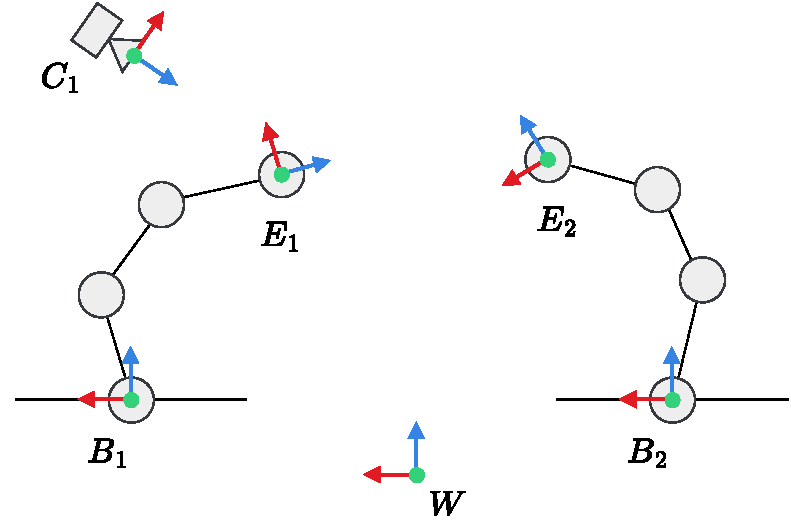
\includegraphics[width=\textwidth]{chapter_1/fig/eye_in_to_hand.pdf}
    \caption{
    Schematic overview of the key coordinate frames of interest for this work. Base-to-base calibration is achieved via two eye-to-hand calibrations. Whilst we show a dual arm system, it is easy to extend the methods discussed in this paper to multiple robots.
    }
    \label{c1:fig:base2base}
\end{figure}
In this section, we formally present the two problems that our research addresses. The key coordinate frames are illustrated in the schematic diagrams shown in \figref{in:fig:eye_to_hand}, and \figref{in:fig:eye_in_hand}, for the eye-to- and eye-in-hand scenarios, respectively. \figref{c1:fig:base2base} adds additional nomenclature for the base-to-base via dual eye-to-hand calibration. The following subsection introduces the notation employed in the entirety of this paper and also states some important assumptions we make to facilitate our approach. 
Subsequently, we outline our problems in the remaining subsections.

\subsection{Notation and Assumptions}
In general, we use 
Greek letters (e.g. $\alpha, \gamma$) to denote scalars, 
Latin letters (e.g. $a, b$) to denote vectors, 
capital letters (e.g. $A, \Gamma$) to denote matrices, and 
calligraphy and blackboard formats (e.g. $\mathcal{A}, \mathbb{B}$) to denote sets and spaces.

\paragraph{Coordinate Frame Transformations} A homogeneous transformation matrix, denoted $\homogeneous{B}{A}\in\mathbb{R}^{4 \times 4}$, represents the pose of frame $A$ with respect to $B$ (i.e. $B$, in this case, is the base frame).
The matrix $\homogeneous{B}{A}$ can be expressed as
\begin{equation}
\homogeneous{B}{A} = 
    \begin{bmatrix}
     R\big({}^{B}q_A\big) & {}^{B}p_A \\
     0_3 & 1
    \end{bmatrix}
    \label{c1:eq:ht}
\end{equation}

where ${}^{B}p_{_A}\in\mathbb{R}^3$ is a column vector representing the position, $R:\mathbb{R}^4\rightarrow\mathbb{R}^{3\times 3}$ is function that converts the unit-quaternion ${}^{B}q_{_A}\in\mathbb{R}^4$ to a rotation matrix, and $0_3$ is the three element row vector containing only zeros.
With reference to the schematic of a robot arm in \figref{in:fig:eye_in_hand}, the camera frame $C$ is expressed in the end-effector frame $E$ by $\homogeneous{E}{C}$, and $E$ is expressed in the robot base frame $R$ by $\homogeneous{R}{E}$. 
%and
%$R$ is expressed in the world frame $W$ by $\homogeneous{R}{R}$.
%Therefore, the camera frame $C$ expressed in the world frame $W$ is found using
%\begin{equation}
%    \homogeneous{R}{C} = \homogeneous{R}{R} \homogeneous{R}{E} \homogeneous{E}{C}.
%\end{equation}

\paragraph{Forward Kinematics} For an $N$-\gls{dof} robot manipulator, the joint positions are denoted $x\in\mathbb{R}^N$. In this work, we assume that the end-effector frame $E$ expressed in the robot base frame $R$, i.e. $\homogeneous{R}{E}$, can be computed accurately using forward kinematics. We denote the relationship between the joint positions and link poses, including the end-effector, by
\begin{equation}
    \begin{pmatrix}
         {}^{R}p_{_L}\\
         {}^{R}q_{_L}
    \end{pmatrix}
    = \phi(x),
    \label{c1:eq:fk}
\end{equation}

where $\phi: \mathbb{R}^N\rightarrow\mathbb{R}^{7}$ represents the forward kinematics function. Given a geometric description of the robot's joints and links (typically in the common URDF format), the forward kinematics $\phi(\cdot)$ is easily derived.

\paragraph{Modality Prerequisites} Regarding the camera, that is either placed in the environment, as in \figref{c1:fig:base2base}, or mounted at the robot end-effector, as in \figref{in:fig:eye_in_hand}, we assume stereo or RGB-D. Finally, we assume access to the mesh files or \gls{cad} models for each of the robot arms.

%\subsection{Robot Base-to-base Calibration}

%In this subsection, we primarily describe the problem associated with \figref{c1:fig:base2base}. As discussed above, several robots could be positioned at once in the operating theater. To enable automated approaches, these robot arms must be aware of the other's position and orientation. With reference to \figref{c1:fig:base2base}, the transforms $\homogeneous{{E_i}}{{R_i}}$ are assumed known for each $i\in[1, 2]$. The goal of this work is to utilize information from the camera located at frame $C$, and with the mesh files or \gls{cad} models to compute estimates for the transforms $\homogeneous{C}{{B_1}}$ and $\homogeneous{C}{{B_2}}$. Given estimates for these frames, we can thus compute one robot pose with respect to the other. This can be expressed by

%\begin{equation}
    %\homogeneous{{B_1}}{{B_2}} = \homogeneous{{B_1}}{C} \homogeneous{C}{{B_2}} = \homogeneous{{B_1}}{C} (\homogeneous{{B_2}}{C})^{-1}
%\end{equation}
%where superscript -1 denotes the matrix inverse. 

%\subsection{Eye-in-hand calibration}

%In this subsection we primarily describe the problem associated with \figref{in:fig:eye_in_hand}.
%Sensors, such as cameras, are often mounted at the robot end-effector in order to perform imaging tasks.
%Often, the transform between the camera frame $C$ and the robot end-effector $E$ is not known.
%Often \gls{cad} models are available for the mount which attaches the camera to the end-effector.
%However, the precise location of the camera imaging sensor is not known accurately, i.e. the camera extrinsic parameters.

%Estimating the unknown static transformation frame $\homogeneous{E}{C}$ is a problem we address in this work as part of our unified approach.
%This is the so-called \textit{eye-in-hand}, or also known as \textit{hand-eye}, calibration problem~\cite{Horaud95}.
%An additional consideration regarding this problem, is that the static transform $\Theta^W_R$ is often also unknown.
%The majority of previous approaches in the literature attempt to solve the ill-posed problem $\Theta^W_C \Theta^R_W = \Theta^E_C \Theta^R_E$.
%Typically, a marker (e.g. checkerboard) of known geometry is affixed to the world frame $W$ that can be estimated and provide an estimate for the transformation frame $\Theta^C_W$ (assuming properly calibrated camera intrinsic parameters).
%As mentioned as an assumption above, the forward kinematics can provide an accurate estimate for the transformation $\Theta^R_E$.
%Multiple images from the camera at various joint positions are taken, and thus recording multiple measurements for $\Theta^C_W$ and $\Theta^R_E$.
%In order to simplify notation, let us denote the unknowns by $X=\Theta^R_W$ and $Y=\Theta^E_C$ and the known values $A_i=\Theta^W_C = (\Theta^C_W)^{-1}$ and $B_i=\Theta^R_E$ (the subscript $i$ refers to the fact that we take multiple measurements), thus the eye-in-hand problem can be re-written as $A_i X = Y B_i$.

%The standard formulation of the eye-in-hand %calibration problem is expressed by
%\begin{equation}
%\label{c1:eq:eyeinhand}
%    \widehat{X}, \widehat{Y} = \underset{X, Y\in\mathbb{R}^{4\times 4}}{\text{arg}\min}~\sum_i \| A_i X - Y B_i\|^2
%\end{equation}
%where $\widehat{X}, \widehat{Y}$ are the solution to the least squares problem and represent estimated homogeneous transformation matrices.
%In our work, we remove the need for a marker affixed in the environment.
%Instead, we make use of the mesh files or \gls{cad} model for the robot arm.
%This requires a reformulation of Equation~\ref{c1:eq:eyeinhand}, which we discuss in later sections.

\section{Materials and Methods}
\label{c1:sec:materials_and_methods}
\begin{figure}[htb]
    \centering
    \includegraphics[width=\textwidth]{chapter_1/fig/hydra_registration.pdf}
    \caption{Detailed point cloud generation and acquisition including pre-processing steps for the proposed robust point-to-plane \gls{icp}. Refers to \secref{c1:sec:robust_icp}.}
    \label{c1:fig:hydra_registration}
\end{figure}

This section introduces a base-to-base baseline calibration procedure in \secref{c1:sec:handshake_calibration}. For the eye-in-hand and eye-to-hand scenario, baselines as introduced in \secref{in:sec:eye_in_to_hand_calibration} are utilized. The baseline calibration procedures are considered the reference for the proposed calibration method. The proposed calibration method is explained in \secref{c1:sec:proposed_calibration_procedure} and an overview is given in \figref{c1:fig:calibration_pipeline} and \figref{c1:fig:hydra_registration}.

In the following sections, homogeneous transforms, from the coordinate frame $A$ to $B$, are denoted through Equation~\ref{c1:eq:ht}
% \begin{equation}
    % \homogeneous{{B}}{A}=\begin{bmatrix} {}^B\mathbf{R}_A & {}^B\textbf{t}_A \\ \mathbf{0} & 1 \end{bmatrix}
% \end{equation}
% where the rotation matrix $^B\mathbf{R}_A$ and the translation vector $^B\textbf{t}_A$.
The world coordinate frame is indicated by $W$. The world coordinate frame $W$ is considered to coincide with the robot base coordinate frame $B$. $W$ and B may thus be used interchangeably. The camera coordinate frame is highlighted through $C$. Furthermore, $A$ indicates the coordinate frame of an ArUco marker.

\subsection{Base-to-base Calibration Baseline}
\label{c1:sec:handshake_calibration}
For the handshake calibration procedure, the two robots are rigidly linked to one another at their end-effectors via a calibration fixture of estimated transform $\homogeneous{{E_1}}{{E_2}}$, see \figref{c1:fig:handshake}. The robots are then moved in admittance control mode and $L$ base-to-end-effector samples are collected for both robots, i.e. $\homogeneous{{B_1}}{{E_1}}^l$ and $\homogeneous{{E_2}}{{B_2}}^l$. Since the system forms a closed kinematic chain, the base-to-base transform $\homogeneous{{B_2}}{{B_1}}$ can then be obtained by minimizing:
%
\begin{equation}
    \label{c1:eq:handsake}
    \min_{\homogeneous{{E_1}}{{E_2}}, \homogeneous{{B_2}}{{B_1}}} \sum_{l=0}^{L-1}\,\homogeneous{{B_1}}{{E_1}}^l\,\homogeneous{{E_1}}{{E_2}}\,\homogeneous{{E_2}}{{B_2}}^l\,\homogeneous{{B_2}}{{B_1}} - I_{4\times4},
\end{equation}
%
where $I_{4\times4}$ is the $4\times4$ identity matrix. Therein, $\homogeneous{{E_1}}{{E_2}}$ is part of the optimization to correct for manufacturing errors.

% Classically, eye-in-hand calibration is conducted by collecting end-effector to base $\homogeneous{B}{E}$ and camera to ArUco marker transformations $\homogeneous{A}{C}$~\citep{eye_in_hand}. The correspondences are re-arranged into an equation of the form $\mathbf{A}\mathbf{X}=\mathbf{X}\mathbf{B}$, with $\mathbf{A}$ containing multiple $\homogeneous{{E_j}}{{E_i}}$ and $\mathbf{B}$ containing multiple $\homogeneous{{C_j}}{{C_i}}$. A 2-step regression is applied to solve for $\mathbf{X}=\homogeneous{{B_2}}{{B_1}}$.

\subsection{Proposed Registration Procedure}
\label{c1:sec:proposed_calibration_procedure}
A high-level overview of the proposed method is shown in \figref{c1:fig:calibration_pipeline}. The method provides an efficient way to find the homogeneous transformation from the robot base frame to the camera frame $\homogeneous{C}{B}$. It aligns an unaligned robot model to an observed instance-segmented point cloud through registration. Importantly, the instance-segmented point cloud and unaligned robot model must be synchronized. The unaligned robot model and the instance segmentation are detailed in \secref{c1:sec:unaligned_robot_model_and_instance_segmented_point_cloud}. 

For the registration step in \figref{c1:fig:calibration_pipeline}, we investigate a simple \gls{icp} algorithm and derive a robust point-to-plane \gls{icp} on a Lie algebra. The simple \gls{icp} variant of the registration procedure is explained in \secref{c1:sec:simple_icp_registration} and the robust point-to-plane \gls{icp} variant in \secref{c1:sec:robust_icp}. A single snapshot is sufficient to find the transformation, which differentiates it from classical calibration procedures described in \secref{c1:sec:handshake_calibration}. In the case of a robot-mounted camera, i.e. eye-in-hand calibration illustrated in \figref{c1:fig:eye_in_hand}, the calibration can be used to determine the transformation from robot end-effector to camera $\homogeneous{C}{E}$. In the case of an externally mounted camera, i.e. eye-to-hand calibration illustrated in \figref{c1:fig:eye_to_hand}, the calibration can be used to determine the robot base-to-base transformation $\homogeneous{{B_2}}{{B_1}}$ through $\homogeneous{{B_2}}{{B_1}} = \homogeneous{C}{{B_2}}^{-1}\,\homogeneous{C}{{B_1}}$.

\subsubsection{Unaligned Robot Model and Instance-segmented Point Cloud}
\label{c1:sec:unaligned_robot_model_and_instance_segmented_point_cloud}
\paragraph{Unaligned Robot Model}
\label{c1:sec:unaligned_robot_model}
To obtain an unaligned robot model, the proposed registration procedure takes as input measured joint positions $x_t$ and link mesh files $\mathcal{M} = \{M_i\}$. Only the mesh vertices $\mathcal{V} = \{V_i\}$ are extracted from the meshes and everything else, e.g. color, is discarded. All mesh vertices $V_i$ are then transformed through $\homogeneous{{L_i}}{R}$, where, given the joint positions, $\homogeneous{{L_i}}{R}$ is obtained via forward kinematics $\phi(x_t)$, see Equation~\ref{c1:eq:fk}. From the transformed mesh vertices $\mathcal{V}$, we sample a total of $N$ points. Therefore, we estimate the volume that each link occupies through its respective bounding box. We then sample $n_i$ points per link vertices $V_i$ via a Poisson-disk sampling strategy, where
\begin{equation}
    n_i = N\frac{b(V_i)}{\sum_j b(V_j)}.
\end{equation}
This sampling strategy guarantees somewhat equally distributed points in space, although future version might only want to perform Poisson-disk sampling over the entire robot.

%Mesh files usually contain interior points, which cannot be observed by the stereo or RGB-D camera. Interior points would indeed confuse the registration discussed in \secref{c1:sec:simple_icp_registration}. To obtain only points that lie on the alpha shape of the mesh, sometimes referred to as the concave hull, we utilize a simple sampling strategy. We specify a bounding box that has the meshes' center of mass at the center. We then uniformly sample N points on the bounding box and for each find the closest point on the mesh. These steps result in in the unaligned robot model, that is the robot model's base frame coincides with the camera coordinate frame.

\paragraph{Instance-segmented Point Cloud}
\label{c1:sec:instance_segmented_point_cloud}
The instance-segmented point cloud is generated by fusing an instance segmentation $S_t$ with a depth map $D_t$ as shown in \figref{c1:fig:calibration_pipeline}. For the instance segmentation, we combine a detector with a segmentor. In this work, a human-in-the-loop acts as the detector by selecting a few points $\mathcal{F}_t$ on the robot in the image. We then deploy the pre-trained \gls{sam}~\cite{Kirillov:arxiv:2023} and prompt it with the detection points $\mathcal{F}_t$. We thus achieve an instance segmentation $S_t$ of the image $I_t$. The depth map $D_t$ can either be obtained via a stereo camera or an RGB-D camera by processing it with a depth estimator. In this work, we utilize Stereolab's Neural Depth perception as the depth estimator. Simply fusing the image segmentation $S_t$ and the depth map $D_t$ then provides the instance segmented point cloud.


% The following sections will explain an \gls{icp} registration on Lie-algebra for said purpose in \secref{c1:sec:robust_icp}. Following that, image-based registration refinements, given a segmentation mask without the need for differentiable rendering are explained in \secref{in:sec:registration_of_3d_point_cloud}.

\subsection{Simple ICP Registration}
\label{c1:sec:simple_icp_registration}
In the case of the simple \gls{icp} we perform single instance registration. The goal is to align the unaligned robot model (as detailled in \secref{c1:sec:unaligned_robot_model}), with the instance-segmented point cloud (as detailled in \secref{c1:sec:instance_segmented_point_cloud}), through finding the transform $\homogeneous{C}{B}$. First, the unaligned robot model $\mathcal{V}_\tau$ is generated (as detailled in \secref{c1:sec:unaligned_robot_model}). Next, robot instances are detected and segmented, which results in the instance-segmented point cloud $P_\tau$. We then compute the instance-segmented point cloud's center of mass for an initial guess of the transform $\homogeneous{{C}}{B,\text{init}}$. Finally, we run an \gls{icp}~\cite{simple_icp} algorithm between vertices $\mathcal{V}_\tau$ and point cloud $P_\tau$, see Equation~\ref{c1:eq:icp}. In contrast to~\cite{simple_icp}, we only consider vertices from $\mathcal{V}_\tau$ whose surface normals point towards the camera. That is, they should be visible to the camera.

\begin{equation}
    \label{c1:eq:icp}
    \text{ICP} = \argmin_{\homogeneous{C}{B}} || \homogeneous{C}{B}(\mathcal{V}_\tau) - P_\tau||_2
\end{equation}

\subsection{Robust Point-to-plane ICP Registration: A Lie Algebra Formulation}
% \subsubsection{Point-to-plane ICP: A Lie Algebra Formulation}
\label{c1:sec:robust_icp}
\begin{algorithm}
\caption{A recap of the robust Lie group formulation of the point-to-plane ICP.}\label{c1:alg:liep2plan}
\begin{algorithmic}
\State Let $\{p\}$ be points to match (the observations). We omit the indices for simplicity here
\State Let $\{q,n\}$ be points with associated normals (the model)
\State Let $t \gets 0$ be a counter for the outer iterations
\State Let $\Theta_0 = \{R_0,T_0\}$ be an initial estimate of the transformation parameters
\While{ICP not converged}
  \State Compute the transformed points $\Theta_t p$
  \State Perform an approximate nearest neighbour search to match $\Theta_t p$ and $q$ points
  \State Discard point pairs associated with distances that are definitely outliers
  \State We now use $i$ indices to indicated matching points
  \State Compute the residuals: $b_i \gets \tilde{n}_i^T (\tilde{q}_i - R_t \tilde{p}_i - T_t)$
  \State \Comment{Previous computation of $\Theta_t p$ should of course be re-used here}
  \State Compute the robust standard deviation: $\sigma \gets \MAD(\{b_i\})/0.6745$
  \State \Comment{Done once to avoid recomputing it in the inner iterations}
  \State Let $\tau \gets 0$ be a counter for the inner iterations
  \State Let $\Theta_{t,0} \gets \Theta_{t}$ be the current estimate of the transformation
  \While{Gauss-Newton not converged}
    \If{$\tau \neq 0$}
      \State Compute the residuals: $b_i \gets \tilde{n}_i^T (\tilde{q}_i - R_{t,\tau} \tilde{p}_i - T_{t,\tau})$
    \EndIf
    \State Compute the robust weights: $\omega_i \gets \omega_{1.345\sigma}(b_i)$
    \State Compute the linear coefficients: $a_i \gets [-\tilde{n}_i^T R_{t,\tau} {{\tilde{p}}_{i\times}}, \tilde{n}_i^T R_{t,\tau}]$
    \State Solve the weighted normal equation:
    \State \quad $\delta\Theta \gets \texttt{chol\_solve}(A^T W A, A^T W B)$
    \State Update the transformation: $\Theta_{t,\tau+1} \gets \Theta_{t,\tau} \cdot \exp(\delta\Theta)$
    \State $\tau \gets \tau+1$
  \EndWhile
  \State Let $\Theta_{t+1} \gets \Theta_{t,\tau}$
  \State $t \gets t+1$
\EndWhile
%\Require $n \geq 0$
%\Ensure $y = x^n$
%\State $y \gets 1$
%\State $X \gets x$
%\State $N \gets n$
%\While{not converged}
%\If{$N$ is even}
%    \State $X \gets X \times X$
%    \State $N \gets \frac{N}{2}$  \Comment{This is a comment}
%\ElsIf{$N$ is odd}
%    \State $y \gets y \times X$
%    \State $N \gets N - 1$
%\EndIf
%\EndWhile
\end{algorithmic}
\end{algorithm}
In the case of the robust point-to-plane \gls{icp}, we capture multiple configurations of the robot. An overview of the method is provided in \figref{c1:fig:hydra_registration}. Deviating from the simple \gls{icp}, \secref{c1:sec:simple_icp_registration}, we dilate the instance segmentations $S_t$ and only keep the boundary regions. Consequentially, we also only keep the boundary regions of the instance segmented point clouds $\mathcal{P} = \{P_t\}$. Similarly to the simple \gls{icp}, we compute the centroids for the instance segmented point clouds $\{P_t\}$ as well as for each robot model $\{\mathcal{V}_t\}$. We then use the Kabsch algorithm to find an initial estimate for the camera to base homogeneous transformation through centroid alignment. Given the initial alignment, we then perform a robust point-to-plane registration on a Lie algebra. 
%We follow the derivation of \chapref{chap:introduction}, \secref{c1:sec:robust_icp}. A summary for which is provided in \algoref{c1:alg:liep2plan}.

% Tom's notes
% \subsubsection{Point-to-plane ICP: A Lie Algebra Formulation}
% \label{in:sec:p2plane}

\paragraph{Basic Formulation}
We first introduce the problem solved by the point-to-plane \gls{icp} algorithm~\cite{Rusinkiewicz:IC3DIM:2001}.
Let $\mathbf{p}_i$ and $\mathbf{q}_i$ be corresponding 3D points in homogeneous coordinates. Let $\mathbf{n}_i$ be a normal vector associated with $\mathbf{q}_i$. We search a rigid body transformation $\mathbf{\Theta}$ in $SE(3)$ that minimizes:
\begin{equation}
\sum_i ||\mathbf{n}_i^T \cdot (\mathbf{\Theta} \cdot \mathbf{p}_i - \mathbf{q}_i)||^2 = \sum_i (\mathbf{n}_i^T \cdot \mathbf{\Theta} \cdot \mathbf{p}_i - \mathbf{n}_i^T \cdot \mathbf{q}_i)^2
\end{equation}

\paragraph{Iterative Optimization on the $SE(3)$ Lie Group}
Let $\mathbf{\Theta}_0$ be the current estimate. In a Lie group iterative optimization approach~\cite{Mahony:JGO:2002,Vercauteren:IPMI:2007}, we seek a perturbation $\Delta\mathbf{\Theta} \in \mathfrak{se}(3)$ composed with
$\mathbf{\Theta}_0$: $\mathbf{\Theta}_1 = \mathbf{\Theta}_0 \cdot \exp(\Delta\mathbf{\Theta})$. We now seek to minimize:
\begin{equation}
\sum_i (\mathbf{n}_i^T \cdot \mathbf{\Theta}_0 \cdot \exp(\Delta\mathbf{\Theta}) \cdot \mathbf{p}_i - \mathbf{n}_i^T \cdot \mathbf{q}_i)^2
\end{equation}

\paragraph{Mathematical Preliminaries}
For convenience, we take advantage of the relationship between the 3D cross product, the Lie bracket on SO(3), and the skew-symmetric matrix operator.
Let $\boldsymbol{\omega} = [\omega_x, \omega_y, \omega_z]^T$ and $\boldsymbol{\eta} = [\eta_x, \eta_y, \eta_z]^T$ be two 3D vectors, we have
\begin{equation}
[\boldsymbol{\omega}, \boldsymbol{\eta}] = \boldsymbol{\omega} \times \boldsymbol{\eta} = \boldsymbol{\omega}_\times \boldsymbol{\eta}
\end{equation}
where
\begin{equation}
\boldsymbol{\omega}_\times =
\begin{bmatrix}
0         & -\omega_z & \omega_y \\
\omega_z  & 0         & -\omega_x \\
-\omega_y & \omega_x  & 0
\end{bmatrix}
\end{equation}

It can be shown that the Lie group exponential in SO(3) admits a closed form through the Rodrigues’ formula. Let us consider $\boldsymbol{\omega}$ as an element of $\mathfrak{so}(3)$, we now have
\begin{equation}
\expl(\boldsymbol{\omega}) = \exp(\boldsymbol{\omega}_\times) = \mathbf{I}^{3\times3} + \frac{\sin(||\boldsymbol{\omega}||)}{||\boldsymbol{\omega}||}\boldsymbol{\omega}_\times + \frac{1-\cos(||\boldsymbol{\omega}||)}{||\boldsymbol{\omega}||^2}\boldsymbol{\omega}_\times^2
\end{equation}
which for small values of $||\boldsymbol{\omega}||$ leads to the following numerically stable approximation
\begin{equation}
\expl(\boldsymbol{\omega}) \approx \mathbf{I}^{3\times3}
+ (1-\frac{||\boldsymbol{\omega}||^2}{6}+\frac{||\boldsymbol{\omega}||^4}{120})\boldsymbol{\omega}_\times
+ (\frac{1}{2}-\frac{||\boldsymbol{\omega}||^2}{24}+\frac{||\boldsymbol{\omega}||^4}{720}))\boldsymbol{\omega}_\times^2
\end{equation}

\iffalse
For compatibility with the 3D cross product, we choose the following basis for the matrix representation of $\mathfrak{se}(3)$:
\begin{align}
e_1 &= 
\begin{bmatrix}
0 & 0 & 0  & 0 \\
0 & 0 & -1 & 0 \\
0 & 1 & 0  & 0 \\
0 & 0 & 0  & 0
\end{bmatrix}
\\
e_2 &=
\begin{bmatrix}
0  & 0 & 1 & 0 \\
0  & 0 & 0 & 0 \\
-1 & 0 & 0 & 0 \\
0  & 0 & 0 & 0
\end{bmatrix}
\\
e_3 &=
\begin{bmatrix}
0 & -1 & 0 & 0 \\
1 & 0  & 0 & 0 \\
0 & 0  & 0 & 0 \\
0 & 0  & 0 & 0
\end{bmatrix}
\\
e_4 &=
\begin{bmatrix}
0 & 0 & 0 & 1 \\
0 & 0 & 0 & 0 \\
0 & 0 & 0 & 0 \\
0 & 0 & 0 & 0
\end{bmatrix}
\\
e_5 &=
\begin{bmatrix}
0 & 0 & 0 & 0 \\
0 & 0 & 0 & 1 \\
0 & 0 & 0 & 0 \\
0 & 0 & 0 & 0
\end{bmatrix}
\\
e_6 &=
\begin{bmatrix}
0 & 0 & 0 & 0 \\
0 & 0 & 0 & 0 \\
0 & 0 & 0 & 1 \\
0 & 0 & 0 & 0
\end{bmatrix}
\end{align}
\fi

Let us consider a 6D vector $\mathbf{u}=[\boldsymbol{\omega};\boldsymbol{\tau}]$ as an element of $\mathfrak{se}(3)$. Its matrix representation is provided by
\begin{equation}
  \mathbf{u}_\dagger =
\begin{bmatrix}
\boldsymbol{\omega}_\times & \boldsymbol{\tau} \\
0  & 0
\end{bmatrix} \in \mathbb{R}^{4\times4}
\end{equation}
which leads to the following closed-form formula for the Lie group exponential for SE(3):
\begin{equation}
\expl(\mathbf{u}) = \exp(\mathbf{u}_\dagger) =
\begin{bmatrix}
\expl(\boldsymbol{\omega}) & L(\boldsymbol{\omega})\boldsymbol{\tau} \\
0  & 1
\end{bmatrix}
\end{equation}
where
\begin{equation}
L(\boldsymbol{\omega}) = \mathbf{I}^{3\times3}
+ \frac{1-\cos(||\boldsymbol{\omega}||)}{||\boldsymbol{\omega}||^2}\boldsymbol{\omega}_\times
+ \frac{||\boldsymbol{\omega}||-\sin(||\boldsymbol{\omega}||)}{||\boldsymbol{\omega}||^3}\boldsymbol{\omega}_\times^2
\end{equation}
where a Taylor expansion should again be used for numerical stability if $||\boldsymbol{\omega}||$ is small:
\begin{equation}
L(\boldsymbol{\omega}) \approx \mathbf{I}^{3\times3}
+ (\frac{1}{2}-\frac{||\boldsymbol{\omega}||^2}{24}+\frac{||\boldsymbol{\omega}||^4}{720})\boldsymbol{\omega}_\times
+ (\frac{1}{6}-\frac{||\boldsymbol{\omega}||^2}{120}+\frac{||\boldsymbol{\omega}||^4}{5040})\boldsymbol{\omega}_\times^2
\end{equation}

\paragraph{First-order Linearization of the Action of the Exponential in $\mathfrak{se}(3)$}
Let $\mathbf{p}=[\tilde{\mathbf{p}};1]$ be a 3D point in homogeneous coordinates. We consider an infinitesimal element $\Delta \mathbf{u}=[\Delta \boldsymbol{\omega};\Delta \boldsymbol{\tau}]$ of $\mathfrak{se}(3)$ and consider the corresponding action on $p$:
\begin{equation}\label{eq:lieactionlinearisation}
\begin{split}
\expl(\Delta \mathbf{u})\mathbf{p} &\approx (\mathbf{I}^{4\times4}+\Delta \mathbf{u}_\dagger)\mathbf{p} = \mathbf{p} +
\begin{bmatrix}
\Delta \boldsymbol{\omega}_\times & \Delta \boldsymbol{\tau} \\
0  & 0
\end{bmatrix} \mathbf{p}
= \mathbf{p} +
\begin{bmatrix}
\Delta \boldsymbol{\omega}_\times \tilde{\mathbf{p}}+\Delta \boldsymbol{\tau} \\
0
\end{bmatrix} \\
&= \mathbf{p} +
\begin{bmatrix}
\Delta \boldsymbol{\omega} \times \tilde{\mathbf{p}}+\Delta \boldsymbol{\tau} \\
0
\end{bmatrix}
= \mathbf{p} +
\begin{bmatrix}
-\tilde{\mathbf{p}} \times \Delta \boldsymbol{\omega} + \Delta \boldsymbol{\tau} \\
0
\end{bmatrix} \\
&= \mathbf{p} +
\begin{bmatrix}
-\tilde{\mathbf{p}}_\times & \mathbf{I}^{3\times3} \\
0 & 0
\end{bmatrix} \Delta \mathbf{u}
= \mathbf{p} + \mathbf{D}(\mathbf{p})\Delta \mathbf{u}
\end{split}
\end{equation}
where
\begin{equation}
\mathbf{D}(\mathbf{p}) = 
\begin{bmatrix}
-\tilde{\mathbf{p}}_\times & \mathbf{I}^{3\times3} \\
0 & 0
\end{bmatrix} \in \mathbb{R}^{4\times6}
\end{equation}

\paragraph{Lie Algebra Linearization of the Point-to-plane Objective}
Plugging \eqref{eq:lieactionlinearisation} in the original point-to-plane ICP cost function we get the following linearization:
\begin{equation}
\begin{split}
\sum_i & \Big(\mathbf{n}_i^T \mathbf{\Theta}_0 \big(\mathbf{p}_i + \mathbf{D}(\mathbf{p}_i)\Delta\mathbf{\Theta} \big) - \mathbf{n}_i^T \mathbf{q}_i\Big)^2
\\
&= \sum_i \Big(\mathbf{n}_i^T \mathbf{\Theta}_0 \mathbf{D}(\mathbf{p}_i)\Delta\mathbf{\Theta} + \mathbf{n}_i^T \mathbf{\Theta}_0 \mathbf{p}_i - \mathbf{n}_i^T \mathbf{q}_i\Big)^2
\end{split}
\end{equation}
Denoting $\mathbf{a}_i = \mathbf{n}_i^T \mathbf{\Theta}_0 \mathbf{D}(\mathbf{p}_i)$, $\mathbf{A}=[\mathbf{a}_0;\ldots;\mathbf{a}_N]$,
$b_i = \mathbf{n}_i^T (\mathbf{q}_i - \mathbf{\Theta}_0 \mathbf{p}_i)$, and $\mathbf{B}=[b_0;\ldots;b_N]$, we end up with a standard linear least squares problem:
\begin{equation}\label{eq:icplls}
||\mathbf{A} \Delta\mathbf{\Theta} - \mathbf{B}||^2
\end{equation}
which can conveniently be expressed using the pseudo-inverse $\mathbf{A}^{\dagger}$ of $\mathbf{A}$:
\begin{equation}
\Delta\mathbf{\Theta} = \mathbf{A}^{\dagger} \mathbf{B}
\end{equation}

In practice, given the dimensions of $\mathbf{A}$, $b$ and $\Delta\mathbf{\Theta}$, \eqref{eq:icplls} is probably best solved by using the normal equations
\begin{equation}
(\mathbf{A}^T \mathbf{A}) \Delta\mathbf{\Theta} = \mathbf{A}^T \mathbf{B}
\end{equation}
and relying on a Cholesky decomposition:
\begin{equation}
\Delta\mathbf{\Theta} = \texttt{chol\_solve}(\mathbf{A}^T \mathbf{A}, \mathbf{A}^T \mathbf{B})
\end{equation}

Note that by expressing $\mathbf{A}$ and $\mathbf{B}$ without homogeneous coordinates, we get:
\begin{equation}
\mathbf{a}_i = [-\tilde{\mathbf{n}}_i^T \mathbf{R}_0 {{\tilde{\mathbf{p}}}_{i\times}}, \tilde{\mathbf{n}}_i^T \mathbf{R}_0] \in \mathbb{R}^{1\times6}
\end{equation}
and
\begin{equation}
b_i = \tilde{\mathbf{n}}_i^T (\tilde{\mathbf{q}}_i - \mathbf{R}_0 \tilde{\mathbf{p}}_i - T_0) \in \mathbb{R}
\end{equation}

\paragraph{Robust Formulation}
To reduce the influence of outliers on the solution, a typical approach is to introduce a
loss function $\rho_\kappa$ parameterized by a scale parameter (a.k.a. soft margin or cut-off) $\kappa$ to scale the residuals. We then seek to minimize:
\iffalse
\begin{equation}
\sum_i \rho\big(\frac{1}{C^2}(\mathbf{n}_i^T \cdot \mathbf{\Theta} \cdot \mathbf{p}_i - \mathbf{n}_i^T \cdot \mathbf{q}_i)^2\big)
\end{equation}

Using the identity loss function $\rho(z)=z$ leads to the original least-squares problem. Classical robust alternatives include:
\begin{description}
  \item[Soft L1]:
  $\rho(z) = 2 (\sqrt{1 + z} - 1)$.
  The smooth approximation of l1 (absolute value) loss. Usually a good choice for robust least squares.

  \item[Huber]:
  $\rho(z) = z \texttt{ if } z <= 1 \texttt{ else } 2\sqrt{z} - 1$.
  Works similarly to ``Soft L1".

  \item[Cauchy]:
  $\rho(z) = \ln(1 + z)$.
  Severely weakens outliers influence, but may cause difficulties in optimization process.

   \item[Arctan]:
   $\rho(z) = \arctan(z)$.
   Limits a maximum loss on a single residual, has properties similar to ``Cauchy".
\end{description}
\fi
\begin{equation}
\sum_i \rho_k\Big(\mathbf{n}_i^T \cdot \mathbf{\Theta} \cdot \mathbf{p}_i - \mathbf{n}_i^T \cdot \mathbf{q}_i\Big)
\end{equation}
or equivalently if we start from a given estimate in the above Lie group setting:
\begin{equation}
\sum_i \rho_k\Big(\mathbf{a}_i \Delta\mathbf{\Theta} - b_i\Big)
\end{equation}
%
Using the square loss function $\rho_\kappa(z)=z^2$ leads to the original least-squares problem. A classical robust alternatives is the Huber loss
\begin{equation}
\rho_\kappa(z) =
\begin{cases}
  z^2 &\texttt{ if } |z| <= \kappa \\
  2|z|\kappa - \kappa^2  &\texttt{ otherwise }
\end{cases}
\end{equation}
with $\kappa=1.345\sigma$ being advocated to provide robustness while retaining appropriate properties when the errors are Gaussian.

This minimisation can be achieved by a standard \gls{irls} approach~\cite{Green:JRSSB:1984} or by including a second order terms in a slightly more advanced reweighted Gauss-Newton approach as discussed in~\cite{Triggs:VisAlg:2000}.
The latter is referred to as the Triggs correction in \footnote{\url{http://ceres-solver.org/nnls_modeling.html\#theory}}. While elegant, previous work has shown that the Triggs correction does not significantly improve on the standard \gls{irls}~\cite{Zach:ECCV:2014,Zach:ECCV:2018}.
Here, for simplicity we thus restrict ourselves to standard \gls{irls}.
Given a choice of scaling factor $\kappa$ and an estimate of the parameters $\mathbf{\Theta}$, the robust problem is converted to a weighted least-squares:
\begin{equation}
\sum_i \omega_\kappa(b_i) ||\mathbf{a}_i \Delta\mathbf{\Theta} - b_i||^2
\end{equation}
with $\omega_\kappa(z) = \rho'_\kappa(z) / z$ being the weight function associated with the Huber loss:
\begin{equation}
\omega_\kappa(z) =
\begin{cases}
  1 &\texttt{ if } |z| <= \kappa \\
  \kappa / |z|  &\texttt{ otherwise }
\end{cases}
\end{equation}

This leads us to the following weighted normal equation:
\begin{equation}
(\mathbf{A}^T \mathbf{W} \mathbf{A}) \Delta\mathbf{\Theta} = \mathbf{A}^T \mathbf{W} \mathbf{B}
\end{equation}
where $\mathbf{W} = \diag\big(\omega_\kappa(b_0), \ldots, \omega_\kappa(b_N)\big)$.

One aspect we haven't addressed yet it the choice of $\kappa$ for the Huber loss. As mentioned earlier, a typical choice is to use $\kappa=1.345\sigma$. We are thus left with the need to robustly estimate the standard deviation of the residuals. This is typically done through a \gls{mad}:
\begin{equation}
\hat{\sigma} = \frac{\MAD(\{b_i\})}{0.6745} = \frac{\median(\{|b_i-\median(\{b_i\}|)\})}{0.6745}
\end{equation}

%% unused section in PhD thesis
% \subsubsection{Registration of a 3D Point Cloud with 2D Stereo Segmentations}
% \label{in:sec:registration_of_3d_point_cloud}
% %
% Let $\mathbf{q}_i$ be 3D points associated to a model object as expressed in an object specific coordinate frame.
% Let $I_L$ and $I_R$ be a pair of stereo images with associated $M_L$ and $M_R$ camera matrices (including both extrinsic and intrinsic).
% We assume that the stereo images are observing the object in an unknown pose $\mathbf{\Theta}$.
% We also assume that the object is relatively textureless and that we do not have a good means of extracting keypoints of interest from the images.
% We however assume that a segmentation of the object in each image can readily be computed, e.g. with the \gls{sam}~\cite{Kirillov:iccv:2023}.
% %
% While differentiable rendering could be used in this context~\cite{Hannemose:SPIE:2019,labbe2021single,Chen:RAL:2023},
% we expect that a simpler algorithm can be designed given the segmentation availability by matching points from 3D to 2D.
% We also expect to potentially gain robustness against illumination and other factors that would impact the appearance of the object in the images.

% Let $S_L$ and $S_R$ be the object segmentation masks in the left and right image respectively.
% We here seek to recover the pose $\mathbf{\Theta}$ such that the projected model points ${M_L \mathbf{\Theta} q}$ match the observed segmentation $S_L$ (respectively ${M_R \mathbf{\Theta} q}$ to match $S_R$).
% Let $\varphi$ be a function to transform from homogeneous to Cartesian coordinates.
% That is $\varphi([x,y,f])=[x/f,y/f]$ and similarly in 3D.
% We can write the objective as:
% \begin{equation}
% \arg\min_{\mathbf{\Theta}} \sum_i
% \min_{p_L|S_L(p_L)=1}|| \varphi\big(M_L \mathbf{\Theta} \mathbf{q}_i\big) - p_L||^2
% + \min_{p_R|S_R(p_R)=1}|| \varphi\big(M_R \mathbf{\Theta} \mathbf{q}_i\big) - p_R||^2
% \end{equation}

% Similar to the approach in~\cite{Fitzgibbon:IVC:2003}, this formulation can be substantially accelerated by taking advantage of the fact that the segmentations are defined on a regular grid. We can thus use a \gls{edt} for which optimized algorithms exist on both \gls{cpu}~\cite{Felzenszwalb:TC:2012}\footnote{\url{https://github.com/cai4cai/distance_transform}} and \gls{gpu}~\cite{Cao:SIGGRAPH:2010}\footnote{\url{https://docs.rapids.ai/api/cucim/stable/api/\#cucim.core.operations.morphology.distance_transform_edt}}.
% Let $\mathcal{D}_{S_L}$ be the \gls{edt} computed from $S_L$ (respectively $\mathcal{D}_{S_R}$ for $S_R$).
% We can now write
% \begin{equation}\label{eq:dt3d2d}
% \arg\min_{\mathbf{\Theta}} \sum_i \mathcal{D}_{S_L}^2\big( \varphi(M_L \mathbf{\Theta} \mathbf{q}_i) \big)
% + \mathcal{D}_{S_R}^2\big( \varphi(M_R \mathbf{\Theta} \mathbf{q}_i) \big)
% \end{equation}

% As in \secref{in:sec:p2plane}, the square loss terms could be replaced by robust alternatives.
% It should further be noted that the evaluation of a distance transform $\mathcal{D}_{S}$ at an arbitrary point $p$ requires the use of an interpolator.
% A typical choice is to rely on bilinear interpolation for which optimized implementations exist on both \gls{cpu} and \gls{gpu}\footnote{\url{https://pytorch.org/docs/stable/generated/torch.nn.functional.grid_sample.html}}.

% Solving for \eqref{eq:dt3d2d} can be done again by taking advantage of the Lie group structure of SE(3). For simplicity, a generic Lie group non-linear least-squares optimizer as found in Theseus\footnote{\url{https://github.com/facebookresearch/theseus}}~\cite{Pineda:NeurIPS:2023} or Ceres\footnote{\url{https://github.com/ceres-solver/ceres-solver}}~\cite{Agarwal:Ceres:2022} can be used.

% It is worth realising that even if a rigid body model is used, formulation \eqref{eq:dt3d2d} may have somewhat trivial solutions if configurations can be found where the projected 2D point set can fit completely inside of the object segmentation mask as this would lead to a zero loss. It may thus be advantageous to somewhat also consider points outside of the model and make sure that these stay outside of the segmentation mask.


%\begin{algorithm}
%\caption{Registration algorithm (refer to \secref{c1:sec:simple_icp_registration} for details). Joint positions $x_t$, images $I_t$, and depth map $D_t$ all correspond to a single configuration, e.g. they are all synchronously observed at time $t=\tau$.}
%\label{alg:registration}
%\begin{algorithmic}
    %\Function{UnalignedRobotModel}{N, $x$, $\mathcal{M}$}
        %\State $\homogeneous{{}}{{}} =$ \Call{ForwardKinematics}{$x$} %\Comment{get link transforms}
        %\State $V =$ \Call{Extract}{$\mathcal{M}$} \Comment{extract vertices from mesh files} 
        %\State $V =$ \Call{Transform}{$\homogeneous{{}}{{}}$, $V$} \Comment{convert mesh vertices by link transforms}
        %\State $V =$ \Call{Sample}{N, $V$} \Comment{sample vertices on robot surface}
%        \State \Return $V$
%    \EndFunction
%    \Function{Registration}{N, $x_\tau$,   $\mathcal{M}$, $I_\tau$, $D_\tau$}
%        \State $\mathcal{V}_\tau =$ \Call{UnalignedRobotModel}{N, $x_\tau$,   $\mathcal{M}$} \Comment{get unaligned robot model}
%        \State $\mathcal{F}_\tau =$ \Call{Detector}{$I_\tau$} %\Comment{detect robot instances}
%        \State $\mathbf{M}_\tau =$ \Call{Segmentor}{$I_\tau$, $\mathcal{F}_\tau$} \Comment{segment robot instances}
%        \State $P_\tau = \mathbf{M}_\tau \odot D_\tau$ %\Comment{compute Hadamard product}
%        \State $\homogeneous{{}}{\text{init}} =$ \Call{CoM}{$P_\tau$} %\Comment{center of mass as initial transform}
%        \State $\homogeneous{C}{B} =$ \Call{ICP}{$\homogeneous{{}}{\text{init}}$, $\mathcal{V}_\tau$, $P_\tau$} \Comment{run iterative closest point}
%        \State \Return $\homogeneous{C}{B}$
%    \EndFunction
%\end{algorithmic}
%\end{algorithm}

\section{Experimental Setup}
\label{c1:sec:experimental_setup}
Two experiments are considered. First, we perform ex-vivo experiments for the simple \gls{icp} algorithm from \secref{c1:sec:simple_icp_registration} in \secref{c1:sec:ex_vivo_experiments}. An overview for the different ex-vivo calibration baselines is given in \figref{c1:fig:calibrations}. Next, we perform in-vivo experiments for the robust point-to-plane \gls{icp} algorithm from \secref{c1:sec:robust_icp} in \secref{c1:sec:in_vivo_experiments}. The in-vivo experimental setup is presented in \figref{c1:fig:in_vivo_setup}.

\subsection{Ex-vivo Experiments}
\label{c1:sec:ex_vivo_experiments}
\begin{figure}[tb]
     \centering
     \begin{subfigure}[b]{0.3\textwidth}
         \centering
         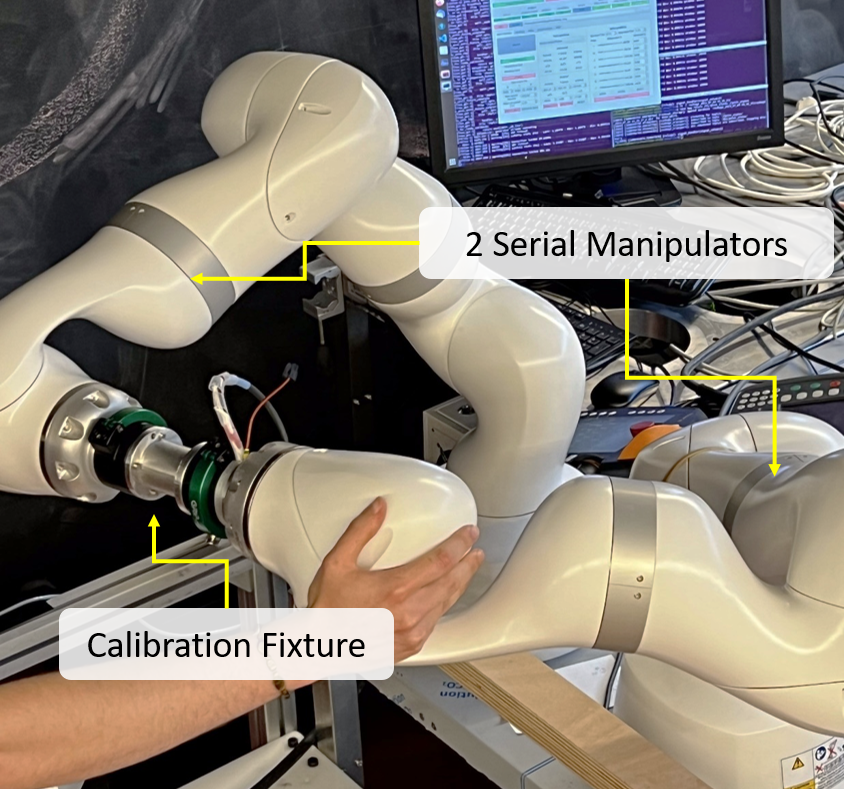
\includegraphics[width=\textwidth]{fig/handshake.png}
         \caption{Handshake calibration for base-to-base calibration. The two serial manipulators are rigidly attached and in admittance control mode.}
         \label{c1:fig:handshake}
     \end{subfigure}
     \hfill
     \begin{subfigure}[b]{0.3\textwidth}
         \centering
         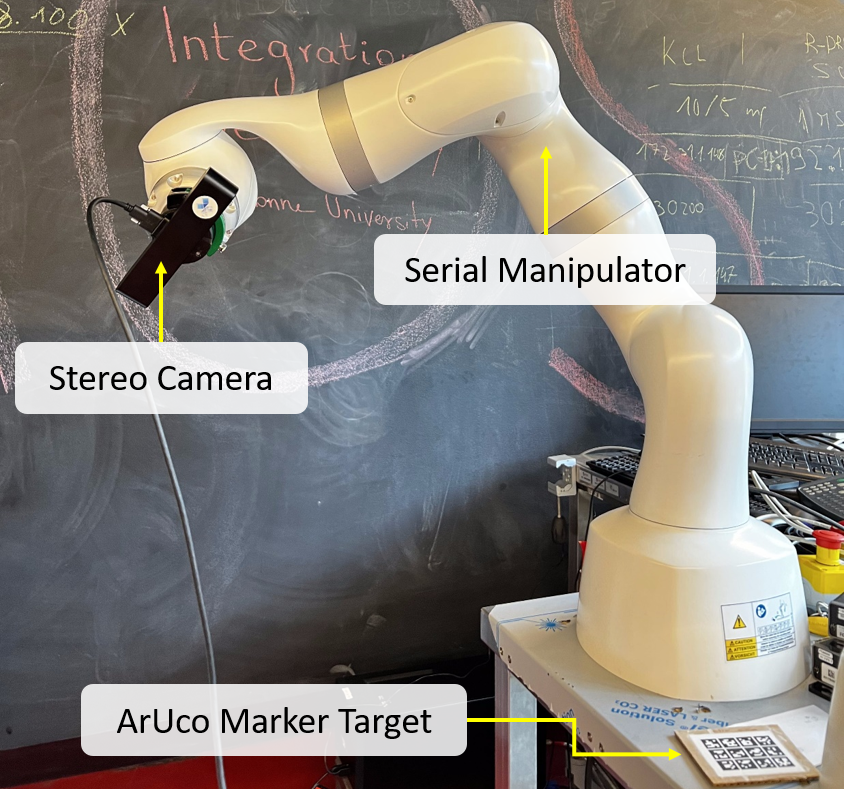
\includegraphics[width=\textwidth]{fig/eye_in_hand.png}
         \caption{Eye-in-hand calibration obtained through self-observation, where the serial manipulator observes itself.\\}
         \label{c1:fig:eye_in_hand}
     \end{subfigure}
     \hfill
     \begin{subfigure}[b]{0.3\textwidth}
         \centering
         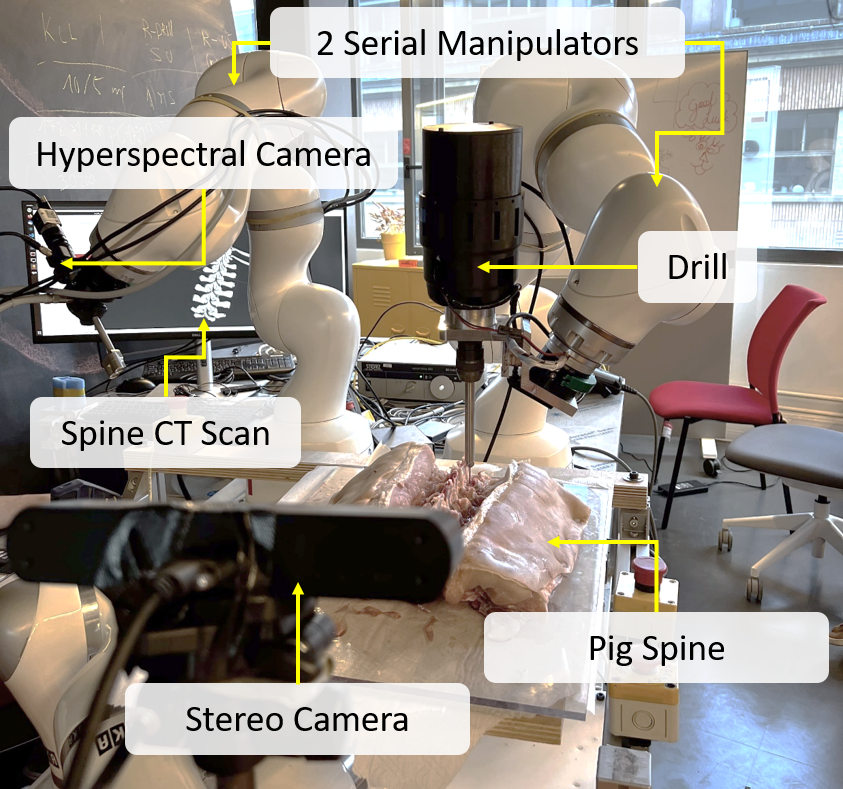
\includegraphics[width=\textwidth]{fig/eye_to_hand.png}
         \caption{Eye-to-hand calibration in a dual serial manipulator setup to obtain base-to-base calibration.\\\\}
         \label{c1:fig:eye_to_hand}
     \end{subfigure}
    \caption{Calibration procedures. The proposed registration procedure, see \figref{c1:fig:calibration_pipeline}, is evaluated against alternative calibrations. The base-to-base calibration via eye-to-hand registration in (c) is compared against a handshake calibration in (a). The eye-in-hand calibration in (b) is compared against a classical calibration via an ArUco marker target, also (b). Refers to \secref{c1:sec:ex_vivo_experiments}.}
    \label{c1:fig:calibrations}
\end{figure}

The experimental setup is shown in \figref{c1:fig:handshake}-\figref{c1:fig:eye_to_hand}. We utilize two KUKA \gls{lbr} Med 7 robots and control them via the \gls{lbr}-Stack~\cite{huber2023lbr} at a control rate of $100\,\text{Hz}$. For the handshake calibration, we deploy them in impedance control mode, see \secref{c1:sec:handshake_calibration}, for all other calibrations we use position control mode. The robots are mounted on a table and are fixed with respect to each other. By construction, their distance is $38\,\text{cm}$. For the camera we use a ZED 2i (Stereolabs, USA). We collect images and depth maps with a resolution of $448 \times 256$ at a frame rate of $15\,\text{Hz}$. For the depth estimation, we utilize the camera in neural depth perception mode.

Four experiments are conducted, two regarding eye-in-hand and two regarding eye-to-hand calibration. For the eye-in-hand calibration, the camera is mounted to the robot via a GRIP G-SHW063 tool connector, see \figref{c1:fig:eye_in_hand}. For the baseline calibration experiments, see \secref{c1:sec:handshake_calibration}, we use a $3\times4$ ArUco marker target of square size $15.77\,\text{mm}$. $1259$ image-joint position correspondences are collected. For the proposed method, see \secref{c1:sec:simple_icp_registration}, we have the robot observe itself through the camera. We collect $1272$ image-joint position correspondences, but only use one. For the eye-to-hand calibration, the camera is put on an external tripod, see \figref{c1:fig:eye_to_hand}. $790$ image-joint position correspondences are collected, again only one is used. Robot 1 and robot 2 are calibrated and the base-to-base calibration is extracted, see \secref{c1:sec:proposed_calibration_procedure}. The base-to-base calibration is compared to a handshake calibration, see \figref{c1:fig:handshake} and \secref{c1:sec:handshake_calibration}. For the handshake, the robots are rigidly connected via a calibration fixture. $27700$ data points are collected of which $277$ are used for the calibration.

\subsection{In-vivo Experiment}
\label{c1:sec:in_vivo_experiments}
\begin{figure}[tb]
    \centering
    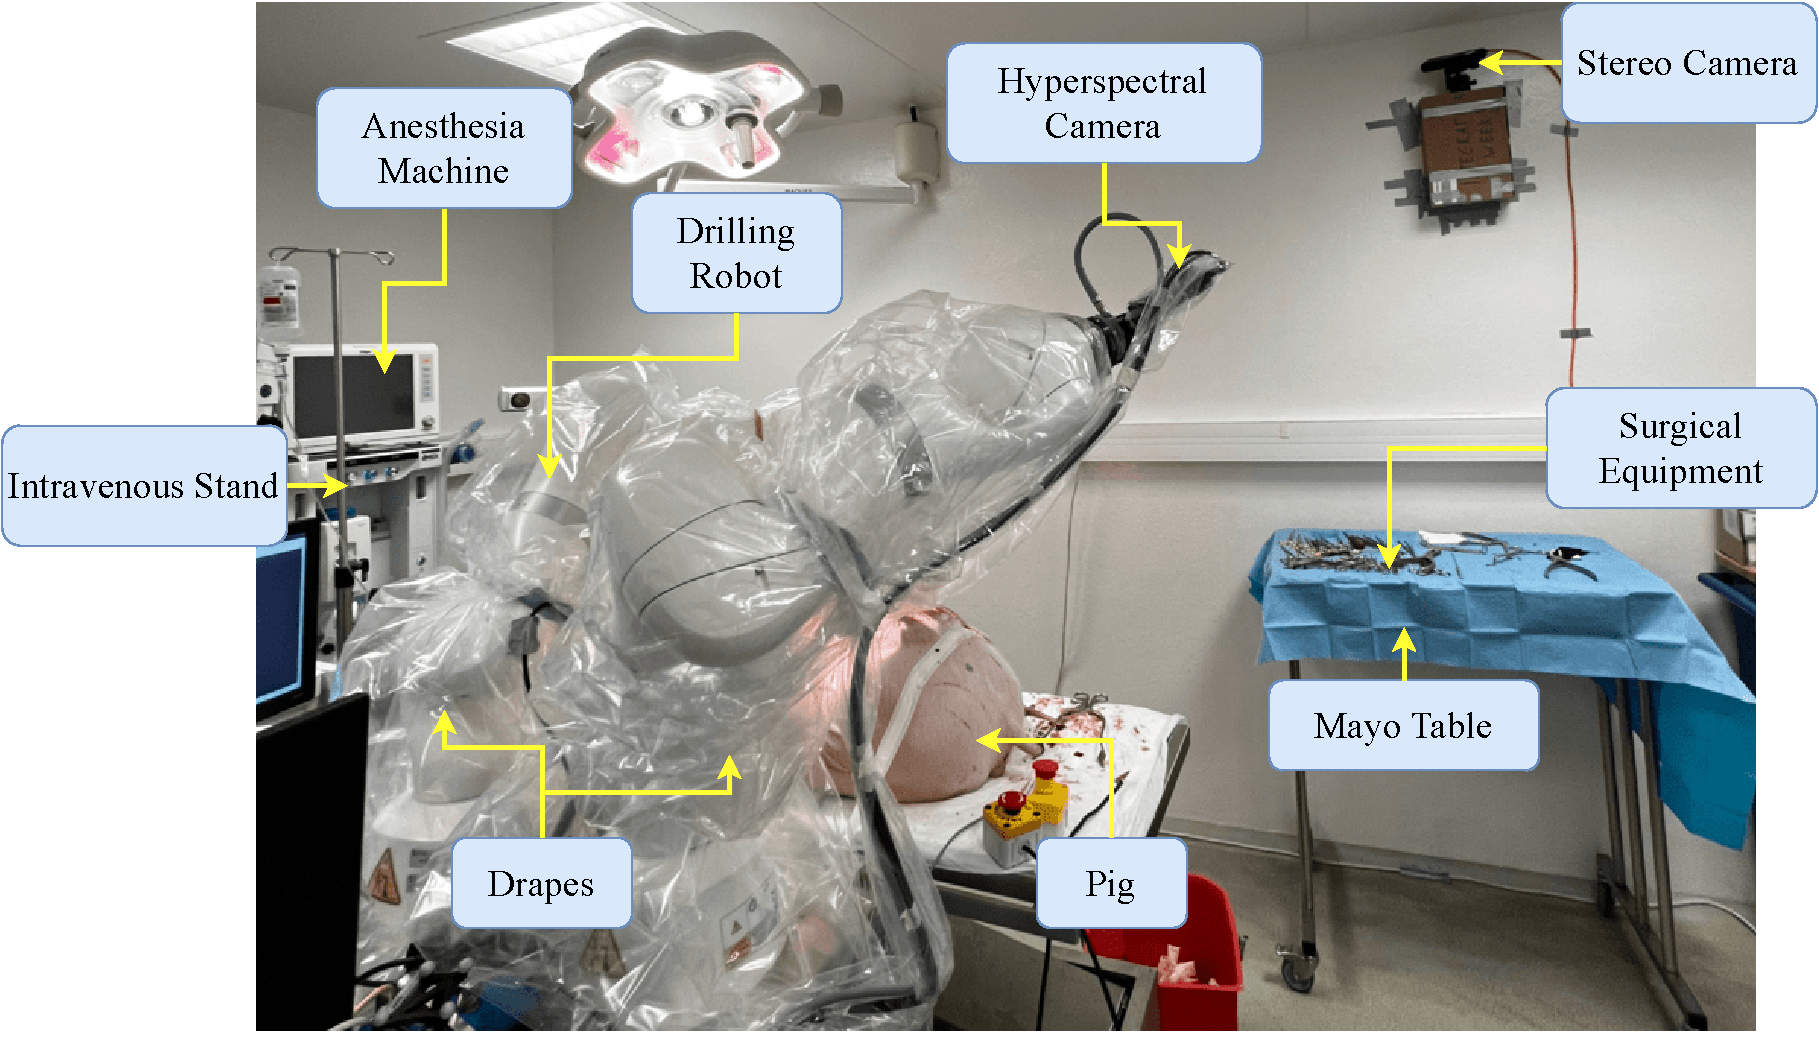
\includegraphics[width=0.8\textwidth]{chapter_1/img/in_vivo_setup.pdf}
    \caption{Clinical setup. A camera is mounted against a wall and both robots are registered using the proposed method of \secref{c1:sec:robust_icp}. Notably, the registration is performed prior to draping. Refers to \secref{c1:sec:in_vivo_experiments}.}
    \label{c1:fig:in_vivo_setup}
\end{figure}
To qualitatively verify the proposed method in a clinically relevant scenario, and to collect data, we conduct an in-vivo study. The primary goal of this experiment, however, is data collection. Given the registration, the recorded data can serve as ground truth for further marker-free registration despite draping. In the study, spine surgery is investigated, and in particular, robot-assisted pedicle screw placement. The pig is put under general anesthesia at all times. An overview of the setup is shown in \figref{c1:fig:in_vivo_setup}. Two KUKA \gls{lbr} Med7 R800 are deployed. Notably, both robots are draped, turning the proposed registration procedure unfeasible. Thus, registration is performed prior to draping, and neither the robots, nor the camera are moved thereafter. A ZED 2i stereo camera (Stereolabs, USA) is wall-mounted, so both robots and the surgical scene are in sight. We record stereo images and depth maps at a resolution of $540 \times 960$. Both robots are put into admittance control mode and are hand-guided into different configurations for sample collection.

\section{Results}
\label{c1:sec:results}
% TODO: cite optas ~\cite{optas} % for control of dual system

\subsection{Ex-vivo Results}
\label{c1:sec:ex_vivo_results}
\begin{figure}[tb]
     \centering
     \begin{subfigure}[b]{\textwidth}
         \centering
         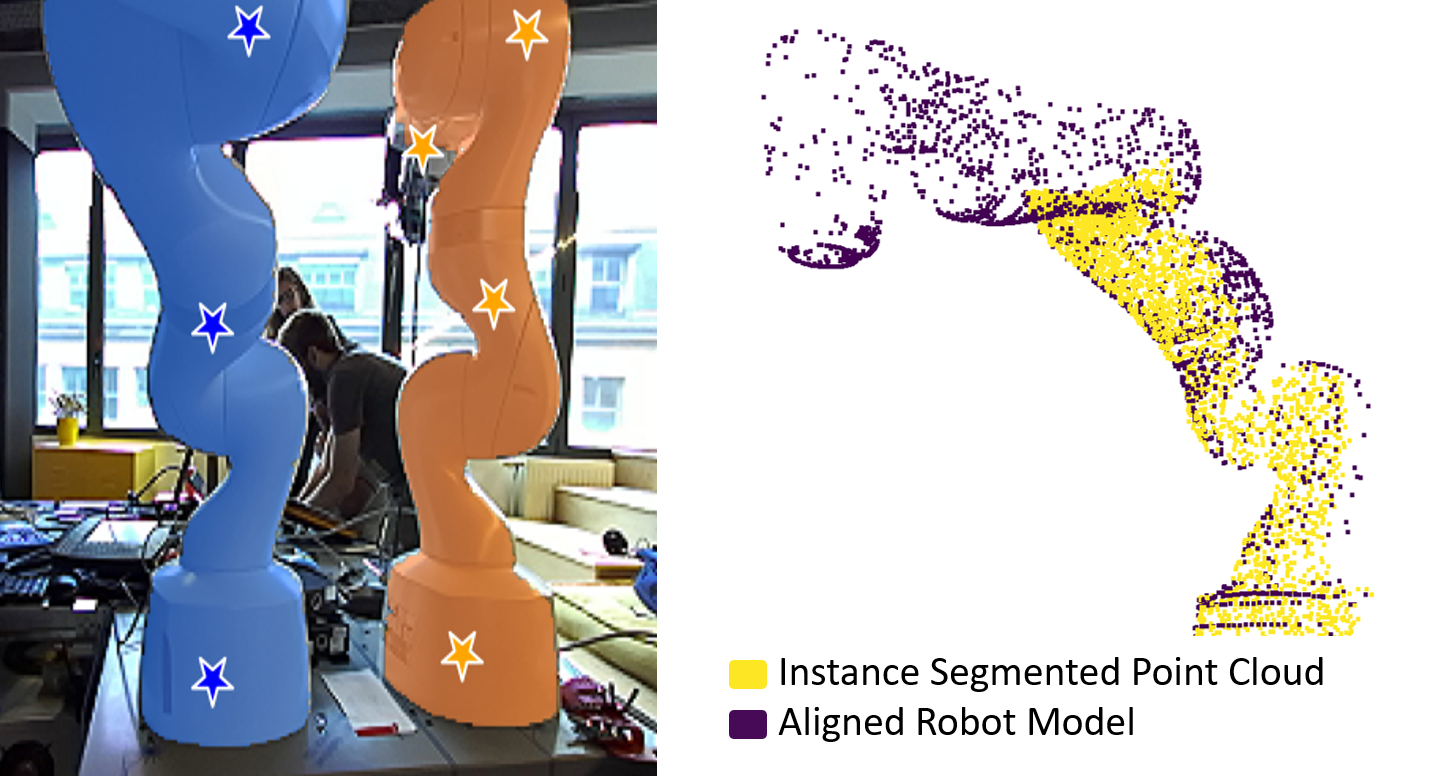
\includegraphics[width=0.6\textwidth]{img/visual_calibration/self_registration_combined_white.png}
         \caption{Eye-in-hand calibration, corresponding to \figref{c1:fig:eye_in_hand}. Left: Instance segmentation. The camera is mounted to robot one, highlighted through the blue mask. For visualization purposes, the image is rotated by $180^{\circ}$. Right: Point cloud to robot model registration.}
         \label{c1:fig:self_registration}
     \end{subfigure}
     \hfill
     \begin{subfigure}[b]{\textwidth}
         \centering
         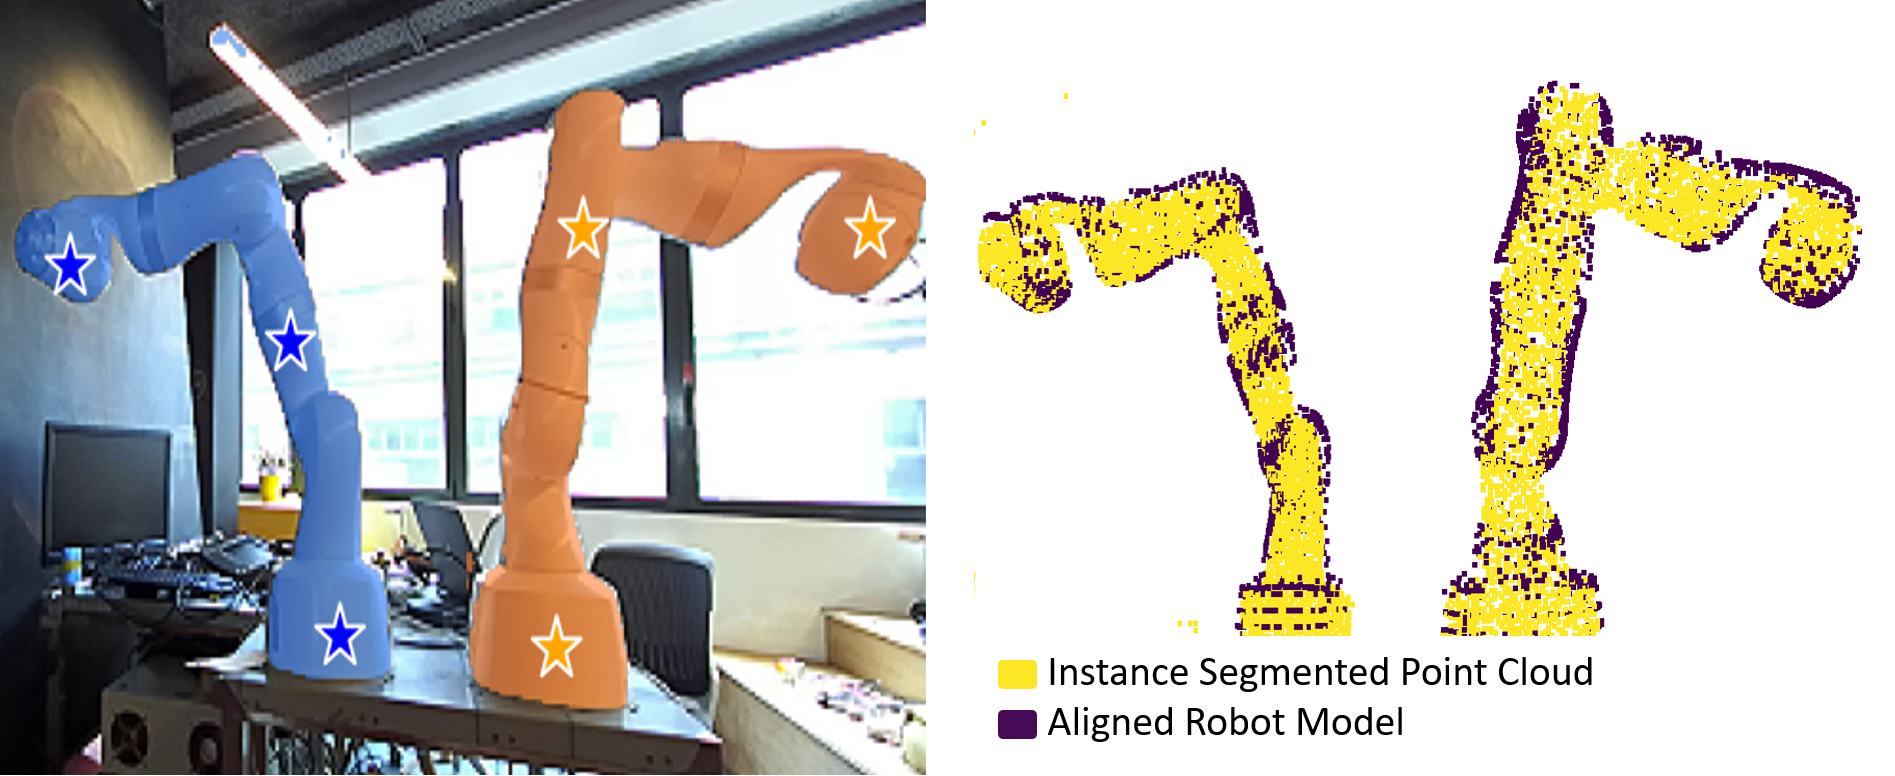
\includegraphics[width=0.6\textwidth]{img/visual_calibration/double_registration_combined_white.png}
         \caption{Eye-to-hand calibration, corresponding to \figref{c1:fig:eye_to_hand}. Left: Instance segmentation. The camera is mounted externally and observes robot one (blue mask) and robot two (orange mask). Right: Point cloud to robot model registration.}
         \label{c1:fig:double_registration}
     \end{subfigure}
     \caption{Ex-vivo eye-in-hand and eye-to-hand registrations. The instance-segmented point clouds $P_\tau$ align well with the robot model $\mathcal{V}_\tau$. Refers to \secref{c1:sec:ex_vivo_results}.}
     \label{c1:fig:registration_results}
\end{figure}
\paragraph{Qualitative Results} The registrations are shown in \figref{c1:fig:registration_results}. It can be observed that in both scenarios, i.e. eye-in-hand (\figref{c1:fig:self_registration}) and base-to-base via eye-to-hand (\figref{c1:fig:double_registration}), the segmentation via initial detection works well. The detections $\mathcal{F}_\tau$ are indicated through stars. Robot one and two can be clearly separated. This precise segmentation $S_\tau$ results in an instance-segmented point cloud with very little outliers. The registration of the unaligned robot models $\mathcal{V}_\tau$ onto the instance-segmented point clouds $P_\tau$ results in a visually compelling alignment (\figref{c1:fig:self_registration} - right - and \figref{c1:fig:double_registration} - right). Therein, the instance-segmented point clouds are visualized in yellow and the aligned robot models are shown in purple.

\paragraph{Quantitative Results} Quantitative results are summarized in \tabref{c1:tab:calibration_results}. For the eye-in-hand calibrations, it can be seen that the classical calibration procedure via ArUco markers deviates significantly from the manufactured values. This is most likely caused by noisy samples. In contrast, the proposed method, although single-shot, compares better with the expected manufactured values, which aligns well with the qualitative results in \figref{c1:fig:self_registration}. For the base-to-base calibration, it should be noted that the robots are fixed on a plain surface. The manufactured values can, therefore, be considered accurate. The proposed method yields precise results along the y-axis (distance between the robots), whereas the handshake deviates by $1\,\text{cm}$. The proposed method deviates $1\,\text{cm}$ along the z-axis from the manufactured and the handshake values. This dimension is the perpendicular offset to the surface plane. It can further be seen that the proposed method deviates slightly from the orientations of the handshake calibrations when compared to the manufactured values. The deviations might be caused by insufficiently synchronized images and joint states.

% NOTE TO SELF:
% classical eye-in-hand calibration seems odd. Only 5 samples were used for registration
% the proposed solution to eye-in-hand seems solid

\begin{landscape}
\begin{table}[htb]
\caption{Calibration results using the proposed method (\secref{c1:sec:proposed_calibration_procedure}) and the baseline methods (\secref{c1:sec:handshake_calibration}). In addition to the calibration baselines, the table also lists manufactured values. The transforms are displayed in terms of translations $t_{x/y/z}$ and rotations in terms of Euler angles $r_{x/y/z}$.}
\label{c1:tab:calibration_results}
\centering
\begin{tabular}{|l|l|l|l|l|l|l|l|l|}
\hline
Calibration Class             & Method       & Transform                                                                                                        & $t_x\,[\text{m}]$ & $t_y\,[\text{m}]$ & $t_z\,[\text{m}]$ & $r_x\,[^\circ]$ & $r_y\,[^\circ]$ & $r_z\,[^\circ]$ \\ \hline
\multirow{3}{*}{Eye-in-hand}  & Manufactured & $\homogeneous{C}{E}$                                                                                  & $ 0.0$            & $-0.06$           & $-0.06$           & $ 0.0$          & $-2.9$          & $-145.0$        \\ \cline{2-9} 
                              & ArUco        & $\homogeneous{C}{E}$                                                                                  & $ 0.0$            & $-0.04$           & $ 0.03$           & $-1.1$          & $-15.0$         & $-167.7$        \\ \cline{2-9} 
                              & Proposed     & $\homogeneous{C}{E}$                                                                                  & $ 0.0$            & $-0.07$           & $-0.08$           & $ 1.6$          & $ 1.6$          & $-146.7$        \\ \hline
\multirow{2}{*}{Base-to-base} & Manufactured & $\homogeneous{{B_2}}{{B_1}}$                                                                           & $ 0.0$            & $-0.38$           & $ 0.0$            & $0.0$           & $0.0$           & $ 0.0$          \\ \cline{2-9}
                              & Handshake    & $\homogeneous{{B_2}}{{B_1}}$                                                                           & $-0.01$           & $-0.37$           & $ 0.0$            & $1.3$           & $0.3$           & $-0.6$          \\ \hline
Base-to-base via eye-to-hand  & Proposed     & $\homogeneous{{B_2}}{{B_1}} = \homogeneous{C}{{B_2}}^{-1}\,\homogeneous{C}{{B_1}}$ & $-0.01$           & $-0.38$           & $-0.01$           & $1.7$           & $2.2$           & $-5.1$          \\ \hline
\end{tabular}
\end{table}
\end{landscape}

% classical eye in hand (huanyu)
% mean translation:
%  [ 0.    -0.042  0.026]
% std translation:
%  [0.159 0.07  0.041]
% mean rotation:
%  [  -1.057  -15.003 -167.708]
% std rotation:
%  [127.06   16.682   6.183]

% inverse of huanyu's
% translation:
%  [-0.015 -0.04  -0.024]
% euler:
%  [  2.199 -14.881 167.56 ]

% proposed
% translation:
% [-0.04  -0.056  0.085]
% euler_c_ee:
% [  0.461   2.212 146.686]

% inverse of proposed
% translation inverse:
% [ 0.    -0.069 -0.084]
% euler_c_ee inverse:
% [   1.601    1.595 -146.655]

% manufactured (zed)
% translation_inv:
%  [ 0.003 -0.06  -0.063]
% euler_inv:
%  [ 0.    -2.865  -156.000 ]

\subsection{In-vivo Results}
\label{c1:sec:in_vivo_results}
\begin{figure}[tb]
    \centering
    \begin{subfigure}[b]{0.49\textwidth}
        \centering
        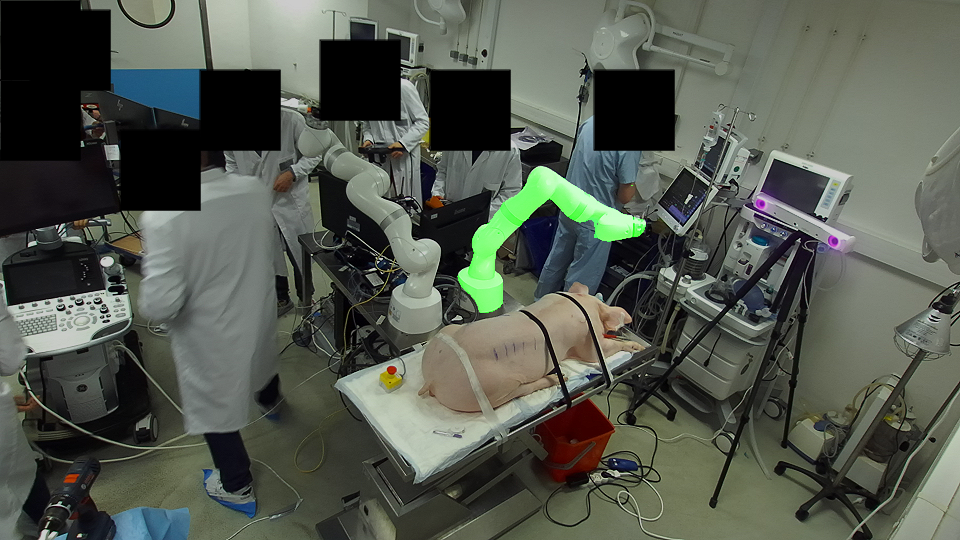
\includegraphics[width=\textwidth]{chapter_1/img/left_mask_overlay_0_anonymized.png}
    \end{subfigure}
    \begin{subfigure}[b]{0.49\textwidth}
        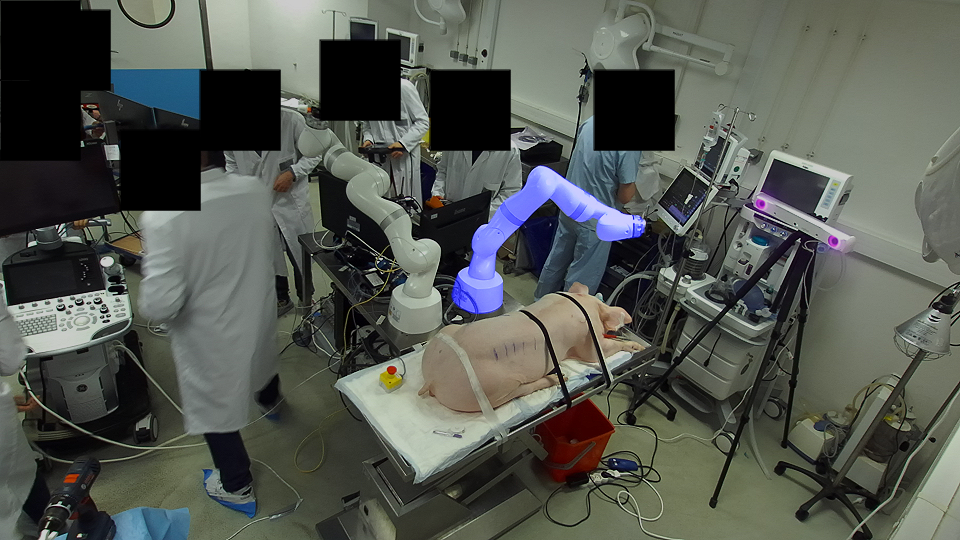
\includegraphics[width=\textwidth]{chapter_1/img/left_render_0_anonymized.png}
    \end{subfigure}
    \caption{Segmented robot (left) and rendered robot given registration (right). Visually, the render shows good alignment with the robot, hinting to an accurate calibration. Refers to \secref{c1:sec:in_vivo_results}.}
    \label{c1:fig:in_vivo_results}
\end{figure}
Initially, we collect 12 measurements for the drilling robot, and 14 measurements for the hyperspecral camera robot. These measurements include joint state, image, and depth correspondences. The positioning of both robots with respect to the camera is shown in \figref{c1:fig:in_vivo_setup}. Using these measurements, we perform a eye-to-hand calibration via the robust point-to-plane \gls{icp}, refer \secref{c1:sec:robust_icp}. 

For both robots, we collect a total of $4588$ stereo frames and depth maps with corresponding joint states, corresponding to about $10$ minutes of data at an average recorded frame rate of $8\,\text{fps}$. We collect an additional $5611$ correspondences for only one robot, either the drilling or the hyperspectral camera robot. This corresponds to about $7$ minutes of data at an average recorded frame rate of $13\,\text{fps}$.

Qualitative results of the registration for the drilling robot are shown in \figref{c1:fig:in_vivo_results}. Therein, and given the registration, we render the robot's meshes into the observed image. The render aligns well with the robot. It should be noted that the segmentation, \figref{c1:fig:in_vivo_results} - left, does not cover the entire robot but misses the bottom left bit. This was the case for all observed drilling robot mask and could be corrected through proper selection of points $\mathcal{F}_t$. For the camera robot on the other hand, we obtain close to perfect instance segmentations $\{S_t\}$. Further exemplary segmentation masks and rendered masks, as well as difference images between segmentation and render, for both, the drilling robot and the camera robot, are shown in \figref{c1:fig:masks}.
\begin{figure}[tb]
    \centering
    \begin{subfigure}[b]{0.32\textwidth}
        
\includegraphics[width=\textwidth]{chapter_1/img/hsi_left_mask_2.png}
        \caption{Camera robot: Segmentation.}
    \end{subfigure}
    \begin{subfigure}[b]{0.32\textwidth}
        
\includegraphics[width=\textwidth]{chapter_1/img/hsi_left_render_mask_2.png}
        \caption{Camera robot: Rendered mask.}
    \end{subfigure}
    \begin{subfigure}[b]{0.32\textwidth}
        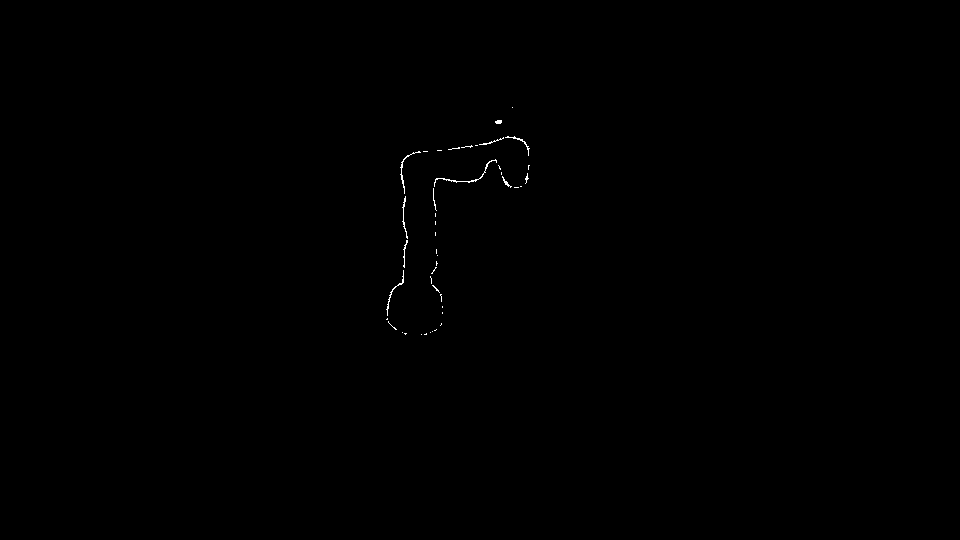
\includegraphics[width=\textwidth]{chapter_1/img/hsi_left_difference_2.png}
        \caption{Camera robot: L1-norm of segmentation and render.}
    \end{subfigure}
    \begin{subfigure}[b]{0.32\textwidth}
        
\includegraphics[width=\textwidth]{chapter_1/img/drill_left_mask_1.png}
        \caption{Drilling robot: Segmentation}
    \end{subfigure}
    \begin{subfigure}[b]{0.32\textwidth}
        
\includegraphics[width=\textwidth]{chapter_1/img/drill_left_render_mask_1.png}
        \caption{Drilling robot: Rendered mask.}
    \end{subfigure}
    \begin{subfigure}[b]{0.32\textwidth}
        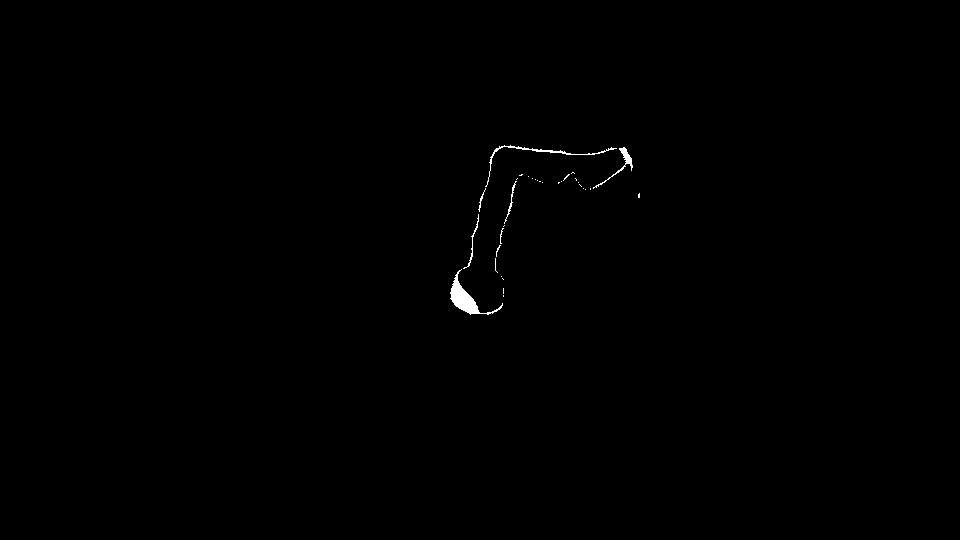
\includegraphics[width=\textwidth]{chapter_1/img/drill_left_difference_1.png}
        \caption{Drilling robot: L1-norm of segmentation and render.}
    \end{subfigure}
    \caption{Example of segmented and rendered masks given the proposed registration procedure. Refer to \figref{c1:fig:in_vivo_setup} for nomenclature. Refers to \secref{c1:sec:in_vivo_results}.}
    \label{c1:fig:masks}
\end{figure}

For the total set of collected samples, we determine the average \gls{iou} between instance segmentations $S_t$ and renders $R_t$. Therein, the \gls{iou} is expressed through
\begin{equation}
    \text{IoU} = \frac{|S_t \cup R_t|}{|S_t \cap R_t|}
\end{equation}
The results are summarized in \tabref{c1:tab:iou}. As can be see, and as already visually observed in \figref{c1:fig:masks}, we find close to perfect average \gls{iou}. For the drilling robot, the average \gls{iou} is slightly worse than for the camera robot. This is because the instance segmentations $S_t$ are systematically off by human annotator.
\begin{table}[tb]
\centering
\caption{Average \gls{iou} of segmented and rendered mask. Also compare to \figref{c1:fig:masks}. Refers to \secref{c1:sec:in_vivo_results}.}
\label{c1:tab:iou}
\begin{tabular}{@{}ll@{}}
\toprule
Robot         & \gls{iou} {[}a.u{]}   \\ \midrule
Camera (left)    & $0.92 \pm 0.01$ \\
Drilling (right) & $0.84 \pm 0.01$ \\ \bottomrule
\end{tabular}
\end{table}

%Drill:
%Average \gls{iou}: 0.8394461441870494
%Std \gls{iou}: 0.013859811026686823
%HSI:
%Average \gls{iou}: 0.9234094580204967
%Std \gls{iou}: 0.009454594255256406

\section{Conclusion and Future Work}% and outlook}
In this work we present a novel vision-based robot calibration procedure that unifies eye-in-hand and eye-to-hand calibration through casting them the same problem formulation. This is achieved by treating the robot as calibration target itself. In the eye-in-hand calibration scenario, the robot simply observes itself whilst in the eye-to-hand scenario the camera observes the robot from an external stand. The introduced formulation can further be used for rapid robot base-to-base calibrations.

\paragraph{Ex-vivo Summary} Promising qualitative results for the simple \gls{icp} (\secref{c1:sec:simple_icp_registration}) are presented in \figref{c1:fig:registration_results}. For both, eye-in-hand \figref{c1:fig:self_registration} and eye-to-hand \figref{c1:fig:double_registration}, the instance-segmented point cloud, as well as the robot model align well after registration. These qualitative observations also solidify through our quantitative comparisons against baselines, which are summarized in \tabref{c1:tab:calibration_results}. Whilst an error remains, the proposed method is much quicker, as it is single shot, is much safer to use, as opposed to the handshake calibration, and does not require any calibration targets, as opposed to the eye-in-hand calibration with ArUco target.

\paragraph{In-vivo Summary} For the in-vivo experiments \secref{c1:sec:in_vivo_experiments}, we deploy an improved version of the registration algorithm, see \secref{c1:sec:robust_icp}. Applicability to a clinical scenario was demonstrated, see \figref{c1:fig:in_vivo_setup}. Visually, we find close to pixel-perfect registrations, see \figref{c1:fig:in_vivo_results}. These visual observations are further confirmed through the measured average \gls{iou}, see \tabref{c1:tab:iou}.
% Given the vast amount of collected data and precise localization, see \secref{c1:sec:in_vivo_results}

\paragraph{Limitations} Shortcomings of this work are that a sufficient view of the robot is required to perform the calibration. In a surgical scenario, draping would cause an insufficient view. Consequentially, the calibration would have to be carried out as initialization and the robots would not be allowed to move afterwards. Clinically, however, it is necessary to drape the robots prior to moving them into position, i.e. prior to moving them into the sterile field.
%Another limitation is the simple \gls{icp} algorithm that was used in \algoref{alg:registration}, \secref{c1:sec:simple_icp_registration}. At times, convergence to local minima is observed.

\paragraph{Future Work} In this work we present a very simplistic registration procedure which already provides highly accurate registration results. These results could immediately be deployed to industrial robots, e.g. for collision avoidance purposes. In the clinical scenario, however, draping is an unsolved issue. Since draping does deform the observed point clouds significantly, the presented method would ultimately fail. However, vast amounts of data and precise localizations were collected as part of the in-vivo study, see \secref{c1:sec:in_vivo_results}. Future work could, therefore, use this data to develop marker-free registration procedures that might function despite draping.

%Improvements could focus on addressing the above, but also on exploring novel concepts. Instead of using a simple \gls{icp} algorithm for registration, one should investigate registration methods that deal well with registering partially observable points clouds. To address the partially observable point cloud issue, one might further move from single shot towards multi shot registration, where multiple robot configurations are observed. This should help improve the calibration accuracy. Research might find that optimal robot configurations exist for performing self-observation in eye-in-hand calibration and also for eye-to-hand calibration. The system might actively sense itself and its surroundings by minimizing uncertainty. Finally, it was omitted in this work that the presented method can also be used to have a robot observe itself and other surrounding robots. Active sensing could be deployed to have an observing robot understand its environment with high precision.
